% This template was originally by R. Jacob Vogelstein
% Updated on March 1, 2010 by Noah J. Cowan
% Updated on May 18, 2014 by Brian Weitzner
% at https://github.com/weitzner/jhu-thesis-template
% Updated on January 29, 2016 by John Muschelli
% at https://github.com/muschellij2/PhD_Thesis
% Updated on April 13, 2016 by Leonardo Collado Torres and
% available at https://github.com/lcolladotor/jhu-thesis-template.
% Forked by John Clayton in December, 2019
% JHU Formatting requirements of Sheridan Libraries may be found at:
% https://www.library.jhu.edu/library-services/
% electronic-theses-dissertations/formatting-requirements/

% The document is based on the standard 12pt LaTeX report class
%\documentclass[12pt,draft]{report}
\documentclass[12pt]{report}

% PDF Creation settings
% \pdfcompresslevel=9
% \pdfminorversion=5
% \pdfobjcompresslevel=2


% Needed to create a PDF/A file
\usepackage[a-1b]{pdfx}

% Incude pdf docs
\usepackage{pdfpages}
% For transferring hyperlinks from PDFs added by pdfpages
% \usepackage{pax}

% For dialect-specific hyphenation etc.
\usepackage[american]{babel}

% T1 font encoding
\usepackage[T1]{fontenc}
% Use UTF8 input encoding
\usepackage[utf8]{inputenc}
%\DeclareUnicodeCharacter{00A0}{ }

% Load latin modern, a font with all the characters
\usepackage{lmodern}

% For generating the dummy text in the mwe template
\usepackage{lipsum}

% Provides various text symbols (such as \textdegree) in TS1 encoding.
\usepackage{textcomp}

% provides ul for cv
\usepackage{soul}

% Set the margins according to JHU specifications
\usepackage{geometry}
 \geometry{
   letterpaper,
   left=1.5in,
   right=1.0in,
   top=1.0in,
   bottom=1.0in}

% Spacing options
\usepackage{setspace}

%Use for indent of first paragraphs
\usepackage{indentfirst}

% Typography and fonts
\usepackage[protrusion]{microtype}
% For multiple columns
\usepackage{multicol}
% for proper text wrapping of nucleic acid sequences
\usepackage{seqsplit}

% Fancy verbatim-like environment for code
\usepackage{listings}
\lstset{basicstyle=\footnotesize\ttfamily,
        columns=flexible,
        breaklines=true
}

% Hyperlink handling
\usepackage[pdfa]{hyperref}
\hypersetup{
   linktocpage,
   unicode,
   colorlinks=true,
   citecolor=link,
   filecolor=link,
   linkcolor=link,
   urlcolor=link
}

% Color handling
\usepackage{xcolor}
%\usepackage{color}

% Color for links
\definecolor{link}{rgb}{0.45,0.51,0.67}

%%% Table of Contents %%%
\usepackage[titles]{tocloft}
% Dots for chapters too
\renewcommand{\cftchapleader}{\cftdotfill{\cftdotsep}}

% To add bibliography to the table of contents
\usepackage{tocbibind}

% Set depth of TOC items
\setcounter{tocdepth}{4}

% Set depth of section numbering
\setcounter{secnumdepth}{4}

\usepackage{calc}
% Tweak to TOC to add 'chapter' to chapter name instead of a number only
\renewcommand{\cftchappresnum}{\chaptername\space}
% Set width of box based on longest label name
\setlength{\cftchapnumwidth}{\widthof{\textbf{Appendix~II~}}}

% Stylize chapter headings
%\usepackage{sectsty}
%\chapterfont{\centering}

% Removes 'Chapter #' title while keeping
% it listed in the TOC
\newcommand\chap[1]{%
  \chapter*{#1}%
  \addcontentsline{toc}{chapter}{#1}}

% Removes 'Section #' title while keeping
% it listed in the TOC
\newcommand\sect[1]{%
  \section*{#1}%
  \addcontentsline{toc}{section}{#1}}

% Removes 'Subsection #'title while keeping
% it listed in the TOC
\newcommand\subsect[1]{%
  \subsection*{#1}%
  \addcontentsline{toc}{subsection}{#1}}

% For oligo table
% Changes dot to hyphen in figure references and captions
\renewcommand{\thetable}{\thechapter-\Roman{table}}
\usepackage{booktabs}
\usepackage{multirow}
\usepackage{longtable}
\usepackage{array}
\usepackage{pdflscape}

% Align on numeric decimal in table
%\usepackage{dcolumn}

% Enhanced control over layout of itemize, enumerate, and description
\usepackage{enumitem}

% Graphics Packages
\usepackage{graphics} 
\usepackage{graphicx}
\usepackage{float}

% Setup style for figure captions
\usepackage[font=small,
            labelfont=bf,
            labelsep=period,
            font=sf,
            hypcap=true]{caption}

% For captions on the side of figures
\usepackage{ifthen}
\usepackage[rightcaption]{sidecap}

% Individual panel captions
%\usepackage{subfig}

% Options for hyperlinking to floats
\usepackage[all]{hypcap}

% Graphics Path
\graphicspath{{Figures/}}

% To change the name of the figures page
\renewcommand{\listfigurename}{Figures}
% To change the default beginning to each line
\renewcommand{\cftfigpresnum}{\bfseries Figure }
% Changes dot to hyphen in figure references and captions
\renewcommand{\thefigure}{\thechapter-\arabic{figure}}
% To change the distance to the start of the figure title
\setlength{\cftfignumwidth}{\widthof{\textbf{Figure~5-10~}}}

% Tikz, for drawing vector graphics
\usepackage{tikz}
\usetikzlibrary{positioning}
\usetikzlibrary{shapes,arrows}

% Enable the glossary
%\makeglossary

% include for Feynman diagrams
\usepackage[compat=1.1.0]{tikz-feynman}

% To add subfigures
\usepackage{subcaption}

% Make appendices
%\usepackage[title,titletoc]{appendix}
\usepackage{appendix}
%\renewcommand{\appendixname}{Appendix}

%%%%%%%%%%%%%%%%%%
% FOR BIBTEX
%%%%%%%%%%%%%%%%%%

% For use with IEEEtran.bst
%\usepackage{cite}
%\usepackage[numbers,square,compress]{natbib}
%\setlength\bibsep{4pt}
% Set bibliography name
%\usepackage{chbibref}
%\renewcommand\bibname{References}

%%%%%%%%%%%%%%%%%%
% FOR BIBLATEX
%%%%%%%%%%%%%%%%%%

\usepackage[
style = nature, 
sorting = none, 
%dashed = false,
%maxbibnames = 99,
backend = biber,
url=false,
isbn=false,
natbib = true
]{biblatex}

% Point to bibfile
\addbibresource{mwe.bib}

% If you want to exclude some portions from the bibliography
%\AtEveryBibitem{
%\clearfield{issn}
%\clearfield{note}
%\clearfield{month}
%}

% Change bib font size
\renewcommand{\bibfont}{\small}

%%%%%%%%%%%%%%%%%%
% DOI from Segmentation (needs hyperref)
%%%%%%%%%%%%%%%%%%

%\makeatletter
%\providecommand{\doi}[1]{%
%  \begingroup
%    \let\bibinfo\@secondoftwo
%    \urlstyle{rm}%
%    \href{http://dx.doi.org/#1}{%
%      doi:\discretionary{}{}{}%
%      \nolinkurl{#1}%
%    }%
%  \endgroup
%}
%\makeatother

% Math
\usepackage{amsmath,amssymb,array}
\usepackage{xspace}


%\newcommand{\bm}[1]{ \mbox{\boldmath $ #1 $} }
%\newcommand{\bin}[2]{\left(\begin{array}{@{}c@{}} #1 \\ #2
%             \end{array}\right) }
% A math shortcut frequently used by John Muschelli
%\newcommand{\bbeta}{\mbox{\boldmath $\beta$}}

%%%%%%%%%%%%% local definitions %%%%%%%%%%%%%%%%%%%%%

\newcommand{\PH}{\ensuremath{H}\xspace}
\newcommand{\Pp}{\ensuremath{p}\xspace}
\newcommand{\PX}{\ensuremath{X}\xspace}
\newcommand{\PZ}{\ensuremath{Z}\xspace}
\newcommand{\PW}{\ensuremath{W}\xspace}
\newcommand{\cPqb}{\ensuremath{b}\xspace}
\newcommand{\cPqt}{\ensuremath{t}\xspace}
\newcommand{\Pqb}{\ensuremath{b}\xspace}
\newcommand{\re}{\ensuremath{e}}


\newcommand{\bbbar}{\ensuremath{b \bar{b}}\xspace}
\newcommand{\Mpl}{\ensuremath{{M_\mathrm{Pl}}}\xspace}% Planck mass
\newcommand{\fbinv}{\mbox{\ensuremath{\,\text{fb}^{-1}}}\xspace}
\newcommand{\TeV}{\ensuremath{\,\text{Te\hspace{-.08em}V}}\xspace}
\newcommand{\Hbb}{\ensuremath{\mathrm{H}\rightarrow\cPqb\overline{\cPqb}}\xspace}
\newcommand{\ttjets}{\ensuremath{\cPqt\overline{\cPqt}}+jets\xspace}
\newcommand{\wjets}{\PW+jets\xspace}
\newcommand{\bjet}{\cPqb~jet\xspace}
\newcommand{\bjets}{\cPqb~jets\xspace}
\newcommand{\sm}{the standard model\xspace}
\newcommand{\mc}{Monte Carlo\xspace}
\newcommand{\com}{13~\TeV\xspace}
\newcommand{\intLumi}{137\fbinv\xspace}

\newcommand{\Hbbt}{double \cPqb\,tagger\xspace}
\newcommand{\Sjbt}{subjet \PQb\,tagger\xspace}
\newcommand{\GRS}{\ensuremath{\mathrm{G}_\mathrm{RS}}\xspace}
\newcommand{\mjjs}{\ensuremath{M_{\textrm jjj}^{\textrm red}}\xspace}
\newcommand{\Mjjs}{\ensuremath{M_{\textrm jjj}^{\textrm red}}\xspace}
\newcommand{\mjj}{\ensuremath{M_{\textrm jjj}}\xspace}
\newcommand{\Mjj}{\ensuremath{M_{\textrm jjj}}\xspace}
\newcommand{\mH}{\ensuremath{M_{\textrm \PH}}\xspace}
\newcommand{\mx}{\ensuremath{M_{\textrm X}}\xspace}
\newcommand{\mux}{\ensuremath{\mu_{\textrm X}^{\textrm CB}}\xspace}
\newcommand{\nsub}{\ensuremath{\tau_{21}}\xspace}
\newcommand{\etaj}{\ensuremath{|\eta|}\xspace}
\newcommand{\deta}{\ensuremath{|\Delta\eta_{\textrm jj}|}\xspace}
\newcommand{\mjp}{\ensuremath{M_{\textrm jet}^{\textrm pruned}}\xspace}
\newcommand{\mjsd}{\ensuremath{M_{\textrm jet}^{\textrm softdrop,puppi}}\xspace}
\newcommand{\mj}{\ensuremath{M_{\textrm jet}}\xspace}
\newcommand{\LambdaR}{\ensuremath{\Lambda_{\textrm R}}\xspace}
\newcommand{\HH}{\PH\PH}
\newcommand{\sgx}{\ensuremath{\sigma_{\textrm X}^{\textrm gaus}}\xspace}
\newcommand{\scbx}{\ensuremath{\sigma_{\textrm X}^{\textrm CB}}\xspace}
\newcommand{\HbbHbb}{\ensuremath{\mathrm{\Hbb\Hbb}}\xspace} 
\newcommand{\XHbbHbb}{\ensuremath{\mathrm{X}\rightarrow\PH\PH\rightarrow\bbbar\bbbar}\xspace}
\newcommand{\mjred}{\ensuremath{M_{\textrm j}}\xspace}
\newcommand{\mred}{\ensuremath{M_{\textrm jj}^{red}}\xspace}
\newcommand{\rpfmc}{\ensuremath{R^\mathrm{MC}_\mathrm{P/F}(\mjred,\mred)}\xspace}
\newcommand{\rpfdata}{\ensuremath{R^\mathrm{data}_\mathrm{P/F}(\mjred,\mred)}\xspace}
\newcommand{\rrat}{\ensuremath{R_\mathrm{ratio}(\mjred,\mred)}\xspace}





%%%%%%%%%%%
% CONTENT %
%%%%%%%%%%%
%
\begin{document}
% Sets paragraph (and not title) spacing, roughly speaking
\setlength{\parskip}{3pt}
\baselineskip=24pt
%
% front matter page numbering
\pagenumbering{roman}
%
% Add title page
% JHU Dissertation title page
\thispagestyle{empty}
% baselineskip of 18pts (i.e. 1.5x spacing or 0.25")
% with 12pt type; 72 points per inch
\baselineskip=18pt
\begin{center}
% Spacer at top of page
\vspace*{3\baselineskip}
%
% TITLE GOES HERE
{\bfseries  PAIRS OF BOOSTED HIGGS \\AND WHERE TO FIND THEM}\\[6\baselineskip]
%
by\\
%
% AUTHOR GOES HERE
D.~Brehm\\[3\baselineskip]
%
%
A dissertation submitted to The Johns Hopkins University in conformity\\
with the requirements for the degree of Doctor of Philosophy\\[4\baselineskip]
%
Baltimore, Maryland\\
% DATE OF SUBMISSION HERE
August, 2021\\[6\baselineskip]
%
% UPDATE THE YEAR HERE
{\copyright{} 2021 D.~Brehm\\
All rights reserved}
%
\end{center}
%
% Reset baseline skip to previous value
\baselineskip=24pt
\newpage 

%
% Setup and add front matter
\pagestyle{plain}
\setcounter{page}{2}
%
% Add abstract
\chap{Abstract}
%
A search is presented for pair production of the standard model Higgs boson using data from proton-proton collisions at a centre-of-mass energy of 13\TeV, collected by the CMS experiment at the CERN LHC in 2016--2018, and corresponding to an integrated luminosity of 137\fbinv. 
The final state consists of two $\cPqb$ quark-antiquark pairs. 
The search is conducted in the region of phase space where at least one pair is highly Lorentz-boosted and is reconstructed as a single large-area jet. 
Depending on the resonance mass, the other Higgs boson may be sufficiently boosted to be also reconstructed as another large-area jet or using two $\cPqb$-tagged jets. 
The results are obtained by statistically combining the analysis channels. Limits on the product of the cross sections and branching fractions are set for narrow and wide bulk gravitons and radions in warped extra-dimensional models having a mass in the range 1000--3000 $GeV$.
Extensions of this search to include Vector Boson Fusion and substituting a Higgs boson for a light scalar Y in the final state of two $\cPqb$ quark-antiquark pairs are also discussed.
New limits are set on the quartic HHVV coupling constant. Expected limits on the mass of the light scalar and heavy resonance interpreted in the context of scalar resonances are presented.
Upper limits are placed on the production cross section of the process as a function of the masses of X and Y.
\clearpage
%
% Add Thesis Readers
\section*{Thesis Readers}
\begin{singlespace}
%
\noindent Dr.~Petar Maksimovic (Primary Advisor)\\
\indent \indent Professor\\
\indent \indent Department of Physics and Astronomy\\
\indent \indent Johns Hopkins University\\

\noindent Dr.~Morris Swartz\\
\indent \indent Professor\\
\indent \indent Department of Physics and Astronomy\\
\indent \indent Johns Hopkins University\\

%\noindent First Lastname \\
%\indent \indent Associate Professor\\
%\indent \indent Affiliation1, and\\
%\indent \indent Department1 \& Department2 at\\
%\indent \indent Johns Hopkins Bloomberg School of Public Health \\
%
\end{singlespace}
%
% Add readers (JHU style is to include readers with in abstract)
%\include{text/03-committee}
%
% Add preface
%\include{text/04-preface}
%
% Add dedication
% Adds a spacer where the header would be
\chapter*{~}
\addcontentsline{toc}{chapter}{Dedication}

\begin{center}
\textit{For Karen.\\
Wit beyond measure is man's greatest treasure.\\[36pt]}
\end{center}
%
% Add acknowledgements
\chap{Acknowledgements}
%\addcontentsline{toc}{chapter}{Acknowledgements}

I first need to thank family for putting up with my academic saga. 
To my Mom and Dad, thanks so much for your unwavering support in helping me finish.
I am sure I would have quit long ago without your help. Your individual examples inspired much of who I am today.
To Kristi, thanks for being willing to step in to my life, even when it was hard, and guide me with your wisdom.
To my siblings, Michael, Zach, Ashley, and Caroline, I appreciate all of the teasing, without which I would not have developed the skin needed to survive this journey.
I also thank you for your friendship. I appreciate everything about being in your lives and look forward to our adventures together in the coming years.
To my grandparents, who gave advice and love and provided environments of peace for me to rest, thank you.

I also had the support of many JHU friends Alice Cocoros, Patrick Bryesse, Rachael Alexandroff, Kevin Nash, Dave Fehling, Keith Redwine, Erini Lambrides, Kirsten Hall, Dan Pfeffer, Tanvi Karwal (pew pew), Kim Berghaus, Charles Hussong, Nikhil Anand, Julian Munoz, Sean Cantrell, and many others who helped me along my way.
I would also like to acknowledge JoVone Pender, Keno Spruill, Matt Collinson, Charles Smith, Kim B. Miller, Debbie Camper and everyone at The Well who helped me when finishing seemed so impossibly hard. I appreciate you all for your love and support. 

I would like to specially recognize a few people. 
Raimon Jackson, thank you for choosing me as a brother and supporting me in my crazy ideas. Thank you for seeing my potential when I could not and fostering it. Thank you for supporting my family when it seemed like it would all fall apart. 
Matt Morris, thank you for your friendship and for all of the joys it has brought. I appreciate all of the time we have spent together and the times you have made my life possible. I hope to be able to return the favor one day.
Marc Osherson, thank you for all that you have given me. From day one, when I was touring JHU with you and the group, I knew we would be friends for life. From working out, discussing builds, drinking beer, and trying to solve the worlds problems, I have been and will remain eternally grateful for your friendship. So sayeth the wise Alaundo!

To my children, Helen and Alice, I hope you look back on my time in grad school with fond memories. I also hope you can forgive any bad temper I may or may not have developed while trying to finish this degree. I love you both very much and look forward to getting to know you as our family adventure continues. 

To Karen, my partner, my love, my light, the smartest person I know, the best mother I could ask for, thank you! Thank you for putting up with late nights, with me hunkering down and forgetting to look up, with commuting an hour and a half one way for 7 years, and for thinking I knew more than you about academia.
I am beyond grateful for the love you have showered me with and am excited to see where the rest of our journey together takes us. I am blessed to wake up with you everyday. Thank you!
%
% To change the name of the contents page
%\renewcommand{\contentsname}{Contents}
%
% Create table of contents
\tableofcontents
%
% Create table list
%\listoftables
%
% Create List of figures
\listoffigures
\clearpage
%
%%% END FRONT MATTER %%%
%
%%%%% MAIN MATTER %%%%%
% Switch page numbering at the end of front matter, before first chapter
\pagenumbering{arabic}
%
%\begin{refsection}[myrefs.bib]
\chapter{The Standard Model of Particle Physics}
\label{chap:intro}

The first recorded use of the word ``elements'' is by Empedocles in the 5th Century B.C. He proposed that 4 substances; earth air, fire, water, make up all of nature and can explain all the complexity of matter. 
This constitutes the first attempt at reductionist thinking in order to explain the world. Reductionist thinking has been very influential in modern physics, especially in the area of particle physics. 
The ability to break down what we previously thought were `` elementary'' particles into the constituent parts has led to many great discoveries. 
The electron, the first truly elementary particle to be discovered, was first hinted at in the 1869 discovery of cathode rays by Johann Wilhelm Hittorf. 
In 1897 , JJ. Thompson showed that cathode rays are streams of a previously unidentified negatively charged particle, which would later be named the electron. 
In 1911, Charles Wilson developed a cloud chamber which allowed for the first photographic evidence of electrons. Protons would be discovered in 1917 and then the neutron would be discovered in 1935. 
This launched a century of discovery that would culminate in 2012 with the discovery of the Higgs Boson, which was one of the last pieces of the puzzle in order to explain 3 of the 4 fundamental forces in nature. We call it the Standard Model of Particle Physics.

The Standard Model(SM) of Particle Physics is the theory that explains all the known particles and the forces that govern their behavior \footnote{With the VERY notable exception of gravity}. 
This is quite an astonishing statement because there are hundreds of known particles and to be able to explain them in a relatively succinct manner is quite the accomplishment of modern science. 
The theory is usually represented in two ways. One, the lagrangian form, see Figure \ref{fig:fig_1-1} \footnote{This is the mathematical expression of the theory from which you can do precise theoretical calculations} and two, a useful diagram that has become popular in explaining the SM, see Figure \ref{fig:fig_1-2}. 
% Figure 1-1
\begin{figure} %  figure placement: here, top, bottom, or page
    \centering
 %   
\includegraphics[width=\textwidth,height=\textheight,keepaspectratio]{fig_2-1}
    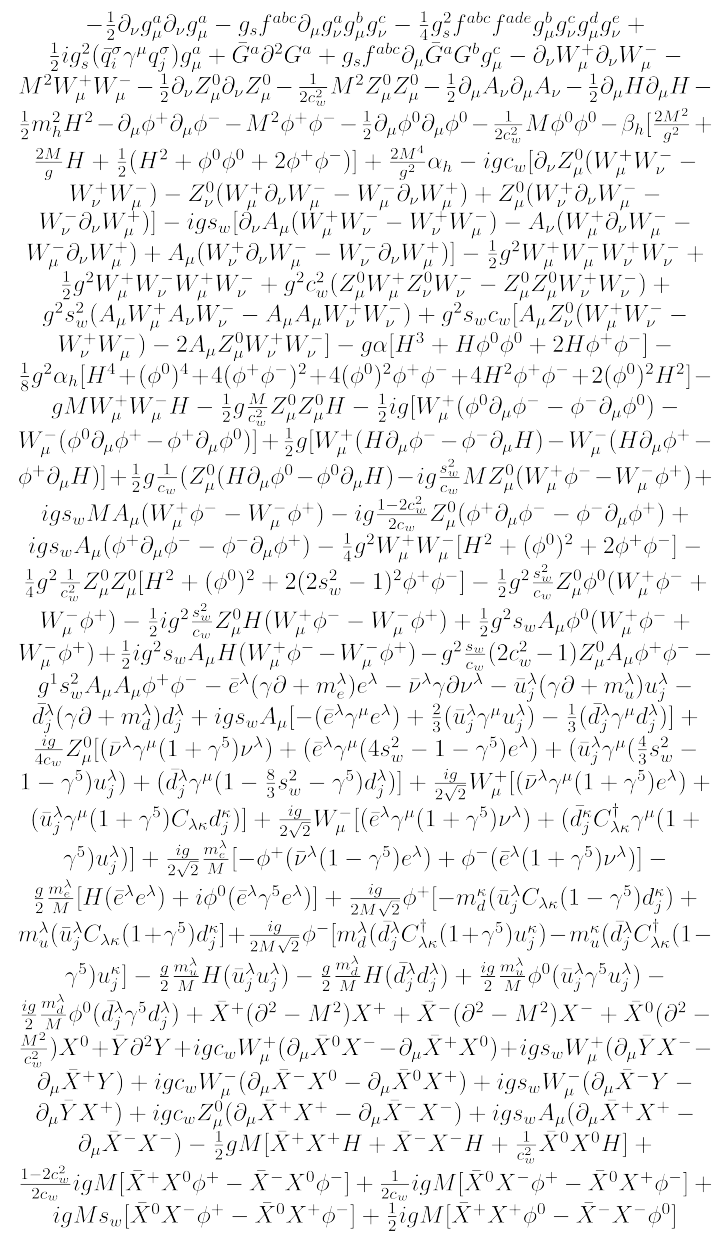
\includegraphics[scale=0.5]{SMlagrangian.png}
    \caption{The lagrangian form of the the Standard Model}
    \label{fig:fig_1-1}
 \end{figure}

 % Figure 1-1
\begin{figure} %  figure placement: here, top, bottom, or page
    \centering
 %   
\includegraphics[width=\textwidth,height=\textheight,keepaspectratio]{fig_2-1}
    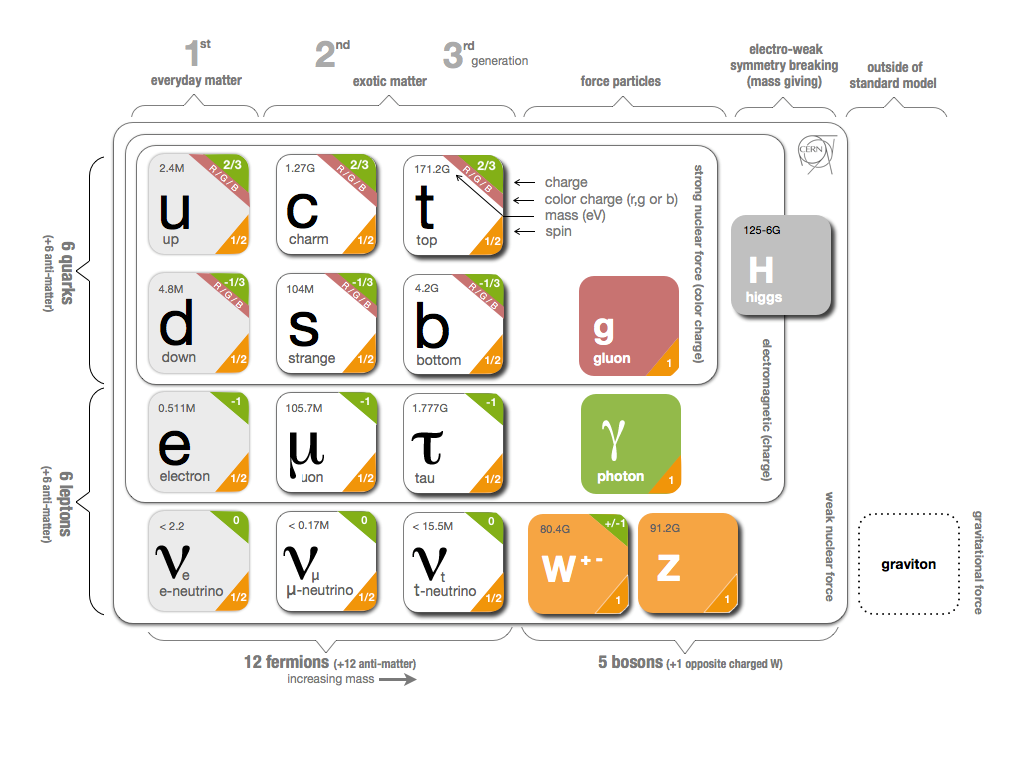
\includegraphics[scale=0.4]{SMinfographic_image.png}
    \caption{A graphical depiction of the Standard Model}
    \label{fig:fig_1-2}
 \end{figure}
\section{Standard Model Particles}
\subsection{Leptons}
Starting with the electron, we can begin to fill out the SM with two other particles that are in some sense just heavier version, the muon ($\mu$) and the tau ($\tau$). 
They all have charge of $-1$ \footnote{The unit of 1 here represents $-1.602$ x $ 10^{-19} Coloumbs$ }. One can see that the muon and the tau have masses roughly 200 and 4000 times that of the electron.
There also exists a pair neutrino, denoted as $\nu$, for each of these leptons which will complete our lepton table in the SM. The electron, muon, and tau neutrinos all have 0 charge and are supposed to be massless in the SM.
You will see that on the table in Figure \ref{fig:fig_1-2} each of the flavors of neutrino have a mass bound of less than some value. This is because various experiments have shown that the neutrinos have some mass.
Since the mass of the neutrino is not predicted by the SM, we expect that some beyond Standard Model (BSM) explanation exists. Each of these particles has an anti-particle which is notated with a bar over the symbol. These are the $\bar{e}, \bar{\mu}, \bar{\tau}, \bar{\nu_{e}}, \bar{\nu_{\mu}}, \bar{\nu_{\tau}}.$

All the leptons also have other properties which are important to mention. The first is something called ``spin'', a vector quantity.
This represents the intrinsic angular momentum of the particle. It is a purely quantum property so you should not think of it as a measurement of how fast the particle rotates. 
Rather it is one component of the total angular momentum of the particle. However, the classical analogy is useful. Just as something can spin in multiple directions classically, this quantum notion of spin has two directions we denote as positive and negative.
This spin can come in quantities of whole units, 0,1,2, and in half units of, $\frac{1}{2}$. The leptons mentioned above all have spin of positive or negative $\frac{1}{2}$, which means they are what we call fermions.

There is another important property which we call helicity (also called handedness). This is defined as the sign of the particles spin vector projected onto its momentum vector.
Usually, negative helicity is referred to as left-handed and positive helicity is referred to as right-handed. This property plays an important part in the calculations of the SM and therefore is not a trivial quantity.
Particles with different handedness can behave differently. For example, while the massive leptons can all be either left or right handed, the neutrinos all left handed and the anti-neutrinos are all right handed.
This phenomenon currently has no explanation in the SM.

\subsection{Hadrons}
There are many more particles that have been discovered in the past 100 years. These have been meticulously detailed in a reference made by the Particle Data Group (PDG) and can be bought in a large textbook form or a small quick reference. 
However, the majority of these particles are composite particles, called Hadrons, that are made up of one of the six quarks seen in Figure \ref{fig:fig_1-2}.
These quarks come in three groupings or ``generations''. \footnote{Why only 3 and not 2 or 4? The SM theory requires 3 generations to preserve its symmetries and properties and indeed this requirement led to the discovery of the 3rd generation of quarks.}
The quarks are the up (u) and down (d), stange (s) and charm (c), and bottom (b) and top (t). The u, c, and t quarks all have charge of $+ \frac{2}{3}$ and the d, s, and b quarks all have charge of $-\frac{1}{3}$.
They have their own masses, spins, and anti-particles (also denoted with a bar over the usual symbol), like the leptons do. They all have spin $\pm \frac{1}{2}$ so they are also fermions.\\

The quarks have an extra property that is unique, called color. This is another quantum property but unlike quantum spin, there is not a very good classical analogy.
It can be thought of as a kind of ``charge'', but it has three different types, red, green, and blue. There also exists anti-red, anti-green, and anti-blue for the anti-quarks.
Unlike electric charge, the color of a quark is not directly detectable and must be determined through the quarks interactions. 
It is also not possible for quarks to exists in anything but color neutral combinations. This will be further explained in the section on forces.
These color neutral combinations make up a lot of the particles you think of today. For example, the proton is made of two u and one d quark. It has a charge of $+1$ because of this fact.
The neutron on the other hand, is made of two d and one u quark. This combinations creates a neutral electric charge. 
Since the quarks always come in color neutral combinations, the fractional charges of the quarks also cannot be directly detected because all of the color neutral combinations also have whole numbers of electric charge.

\subsection{Bosons}
There are 5 bosons listed in figure \ref{fig:fig_1-2}. They are the photon, the gluon, the $W^{\pm}$, the Z and the Higgs bosons.
Unlike the fermions, which all have spin $\pm \frac{1}{2}$, the bosons all have a unit spin of 1\footnote{There exists the theoretical possibility of spin 0 or 2 bosons but none has been detected so far}.
The photon and the gluon are massless, while the W, Z, and Higgs bosons have mass. This is not an accident and will be further explained in the following section on forces. So why do we distinguish fermions from bosons?
The reason is that they fundamentally behave differently. The fermions are the stuff that everyday matter is made of but the bosons are what mediate the interactions between fermions. 
To put it simply, the bosons act on the fermions in what we call the forces of the SM.\\

\section{Standard Model Forces}
There are three fundamental forces that the SM explains, electromagnetism, the weak force, and the strong force. You will note the obvious absence of gravity.
While gravity was the first force to be quantified in Newton's 3 Laws, it has resisted our attempts at understanding it at a quantum level. Many famous, and not famous, physicists have worked tirelessly to find a resolution to this problem.
To date, our inability to reconcile the current theory of gravity with the quantum nature of the SM is one of the most vexing problems facing physics.

The forces of the SM are mediators between particles. It is therefore useful to discuss how this is done mathematically. 
We can consider a very basic situation where two particles are launched at each other. Let us consider like charges so that the two particles will repel each other.
Then we can construct an infinite sum of all the possible interactions between the two particles that start in an initial state, $i$, and end in some final state $f$ as:
\begin{equation}
S_{i \rightarrow f} = \sum_{n=0}^{\inf} I^{n} 
\end{equation}
where each term $I^{n}$ is a different possible interaction between the two particles. The first term is not interesting because it is the term that denotes the two particles not interacting.
So the first interacting term is then:
\begin{equation}
I^2 =  (\pm)^n \bar{\psi(x)} V \psi(x)\bar{\psi(x')} V \psi(x') \int (\frac{dk}{2 \pi})^4 \frac{-g_{\mu \nu}}{k^2 - i0} e^{-ik(x-x')}
\label{eq:eq_baseIntegral}
\end{equation}
where the terms $\psi, \bar{\psi}$ refer to the two particles initial and final states and the V term is the interaction vertex. 
The $\frac{g_{\mu \nu}}{(k^2 - i0)}$ term in the integral is propagator which denotes the force interaction between the two particles (in this case we are mediating the electromagnetic force with a photon). The integral is computed over all incoming and outgoing momenta, $k$.
\\

\begin{figure} %  figure placement: here, top, bottom, or page
   \centering
      \feynmandiagram[horizontal=a to b] {
      i1  [particle=$\phi$] -- [fermion] a -- [fermion] i2  [particle=$\phi$],
      a -- [photon, edge label=\(\gamma\),] b,
      f1 [particle=$\bar{\phi}$] -- [fermion] b -- [fermion] f2 [particle=$\bar{\phi}$],
      };
   \caption{An example Feynman Diagram}
   \label{fig:fig_1-3}
\end{figure}


This equation, while precise and useful for direct computation, is not very instructive and can be put in a pictorial representation that is much easier to read.
These representations are called Feynman Diagrams. Each term in the infinite sum above can be drawn with a Feynman diagram allowing us to see all the necessary components for the interaction.
This allows us to look at specific physical processes without having to resort to long equations.
More importantly, this representation does not lose any of the preciseness of the equations, they are essentially one and the same. 
\begin{equation}
   \feynmandiagram[inline=(d.base),horizontal=d to b] 
   {a -- [fermion] b -- [fermion] c,b -- [boson] d [particle=\(\gamma\)],
   };
   = V
   \label{eq:eq_Vertex}
\end{equation}
Equation \ref{eq:eq_Vertex} is the mathematical expression for a vertex. A vertex is essentially the interaction point between two particles.
One can build the diagram in Figure \ref{fig:fig_1-3} by combining two vertices and correctly writing the corresponding propagator.

Physically, what is happening is that two particles are coming together, combining into an intermediate particles, and then that intermediate particle is decaying into two particles.
This general description is actually very powerful. One can construct any number of particle combinations in such a way as they annihilate (or merge) into an intermediary particle and then decay into two (maybe even more) new particles. 
This ability to write down particle interactions based on a set of rules, which we will describe in following sections, is the foundation of the SM. We can classify three of the four fundamental forces of nature by constructing rules around the combination of vertex diagrams with particular intermediate particles.
These intermediate particles are usually the bosons that govern a force that the particles are interacting with each other through. 


\subsection{Electromagnetic Force}
Classically, Maxwell's equations do a very good job describing electromagnetism. However, in the quantum realm they do a poor job. The quantum theory of electromagnetism is called 
\textit{quantum electrodynamics}. This theory governs all of the possible interactions between the photon, the propagating particle of the electromagnetic force, and any particle that interacts with the photon.
Recall that the interaction vertex is the base of the rules for constructing Feynman diagrams and the interaction vertex for the photon is given in equation \ref{eq:eq_EMVertex} as:
\begin{equation}
   \feynmandiagram[inline=(d.base),horizontal=d to b] 
   {a -- [fermion] b -- [fermion] c,b -- [boson] d [particle=\(\gamma\)],
   };
   = i e \gamma^{\mu}
   \label{eq:eq_EMVertex}
\end{equation}
The equation for the propagating photon is:
\begin{equation}
   \gamma =  \frac{g_{\mu \nu}}{(k^2 - i0)}
\end{equation} 
which when combined together and integrated over all momenta, can be made into an equation which is similar in form to \ref{eq:eq_baseIntegral}.

A quick example of how powerful these tools can be is electron-positron annihilation. If a positron and an electron interact through a photon we will get the diagram shown in Figure \ref{fig:fig_1-4}.
We can also use some rules from classical electromagnetism, i.e charge is conserved, to tell us if this will actually happen in real life. In this example, the total charge of the incoming particles is $1 + (-1) = 0$. 
The photon has charge $= 0$ so then this will conserve charge and is possible in nature. Using charge conservation as another rule we can construct other diagrams by just switching out the electron-positron pair with another lepton, anti-lepton pair.
One classic example is to use the muon and anti-muon which yields the diagram seen in Figure \ref{fig:fig_1-5}. QED is very well tested in modern day experiments and there are no known expected differences between it and the SM.


\begin{figure} %  figure placement: here, top, bottom, or page
   \centering
      \feynmandiagram[horizontal=a to b] {
      i1  [particle=$e^{-}$] -- [fermion] a -- [fermion] i2  [particle=$e^{+}$],
      a -- [photon, edge label=\(\gamma\),] b,
      f1 [particle=$e^{+}$] -- [fermion] b -- [fermion] f2 [particle=$e^{-}$],
      };
   \caption{Electron positron annihilation.}
   \label{fig:fig_1-4}
\end{figure}

\begin{figure} %  figure placement: here, top, bottom, or page
   \centering
      \feynmandiagram[horizontal=a to b] {
      i1  [particle=$e^{-}$] -- [fermion] a -- [fermion] i2  [particle=$e^{+}$],
      a -- [photon, edge label=\(\gamma\),] b,
      f1 [particle=$\mu^{+}$] -- [fermion] b -- [fermion] f2 [particle=$\mu^{-}$],
      };
   \caption{Electron positron annihilation into a muon and anti-muon pair.}
   \label{fig:fig_1-5}
\end{figure}

\subsection{Strong Force}

The Strong Nuclear Force, or strong force for short, governs the interactions inside of hadrons like the proton and neutron. The mediator, or propagator, for the strong nuclear force is the gluon. The theory governing this force is called \textit{Quantum Chromodynamics}.
It can be said that QED is the theory of electrically charged interaction and the analogy for QCD is that it is the theory for colored interactions \footnote{recall that I described quarks as having a color charge.}.
Unlike the photon, which since it has no charge it cannot couple to itself, the gluon has a color charge and so the interaction vertices possible to make Feynman diagrams are slightly more complicated and are shown in Figure \ref{fig:fig_1-6}.
\begin{figure} %  figure placement: here, top, bottom, or page
   \centering
   \begin{subfigure}[t]{0.49\textwidth}
      \feynmandiagram[horizontal=a to b] {
         i1  [particle=quark] -- [fermion] a -- [fermion] i2  [particle=quark],
         a -- [gluon, edge label=gluon] b, 
      };
   \end{subfigure}
   \feynmandiagram[horizontal=a to b][edges = gluon] {
         i1  [particle=gluon] --  a --  i2  [particle=qluon],
         a -- [gluon, edge label=gluon] b, 
      };
   \begin{subfigure}[t]{0.49\textwidth}
      \feynmandiagram[horizontal=a to b][edges = gluon] {
         i1  [particle=gluon] --  a --  i2  [particle=qluon],
         f1 [particle=gluon] -- a --  f2 [particle=gluon], 
      };
   \end{subfigure}

   \caption{Strong force Vertices.}
   \label{fig:fig_1-6}
\end{figure}
Just like in QED, if we apply a conservation law we can constrain what diagrams we can draw. However, unlike with QED, the color charge is not as straight forward.
For the diagrams in Figure \ref{fig:fig_1-6} to work, we need each gluon to carry one color and one anti color since each quark carries only a color or anti color.
Naively, one might think to just combine a color anti color pair like red anti-red, but gluons cannot carry both the color and corresponding anti color.
This is due to the nature of the behavior of the strong force. 

To give a little more context, protons and neutrons (sometimes called nucleons to refer to both of them) are confined to the nucleus by the strong force.
However, they do not carry color charge in the same way that quarks do. The distinction here is that while the gluon is force carrier particle binding the quarks together inside the nucleons, it does not do that between nucleons.
Two quark combinations called mesons are the mediators between nucleons. This difference is due to the emergent properties of complex systems of colored particles and is sometimes called the \textit{residual strong force}. 
Since the mesons are not massless, the range for which the strong force can be felt is much smaller than say electromagnetism. In the case of these nucleons, they form what is called a color singlet. 
The color singlet is the superposition of quantum states as:
\begin{equation}
   \frac{r \bar{r} + b \bar{b} + g \bar{g}}{\sqrt{3}}
\end{equation}
Singlet states interact with each other. This allows us to make an empirically driven statement that since the gluon is massless, and force mediated by the singlet state has a range limit, no gluons will carry this color singlet state.
This then allows us to construct the remaining color combinations for the gluons. There are eight of them and so they are called the color \textit{octet}.
The are as follows:
\begin{gather}
   \frac{r \bar{b} + b \bar{r}}{\sqrt{2}} \quad \frac{r \bar{g} + g \bar{r}}{\sqrt{2}} \quad \frac{b \bar{g} + g \bar{b}}{\sqrt{2}} \quad \frac{r \bar{r} + b \bar{b}}{\sqrt{2}} \nonumber\\
   \frac{-i(r \bar{b} + b \bar{r})}{\sqrt{2}} \quad \frac{-i(r \bar{g} + g \bar{r})}{\sqrt{2}} \quad \frac{-i(b \bar{g} + g \bar{b})}{\sqrt{2}} \quad \frac{r \bar{r} + b \bar{b} - 2g \bar{g}}{\sqrt{6}}
   \label{eq:eq_colorOctet}
\end{gather}
Interestingly, this is not just the only set of possible combinations, but it is also the least complex. One might ask, well what if I have sufficient energy to force something into a color singlet state?
This becomes an interesting questions because physics not only prevents this from happening but does so in a way that allows us to further explore the SM.\\

For the sake of argument, lets say we smashed an electron and proton together with enough energy that one of the quarks in the proton was ejected.
Any other parts of the proton that are ejected as well will interact through the strong force also. As the constituent quarks drift, the gluons that had bound them inside the proton form a web of self interacting connection called the color tube.
These tubes exert constant force when stretched and increase in energy until they reach a characteristic size where it become more energetically favorable to create two new quarks out of the vacuum.
This means that the lone quark that we ejected out of the proton will at the distance of about $10^{-15}$ meters, roughly the radius of atomic nuclei, become a new bound state meson because the lone quark cannot be in a color singlet state. 
If the quark still has too much energy to be bound in the meson, the process continues creating new quark anti quark pairs out of the vacuum until all free quarks are in bound states.
This property is called \textit{confinement} and the method by which the new quarks are produced in the vacuum is called \textit{hadronization}. 
Hadronization in particular is important because it creates objects called ``jets'' which will be crucial to our experiment.


\subsection{Weak Force}

When we say the very early universe was very hot, what we mean is that the ambient temperature was extremely hot because of how energetic the particles were during that time.
During this time, the electromagnetic force was unified with what we know as the weak nuclear force into what is called the Electroweak interaction. This force was mediated by 4 massless bosons named $W_1$, $W_2$,$W_3$, and $B$. 
Another field that matters in this story is the Higgs field which will be more completely described in the following section. At these high energies, the 4 original bosons did not interact with the Higgs field. However, as the universe cooled, this picture changed.
As these original 4 bosons started interacting with the Higgs field, their interactions with the fermions changed. The fermions would no longer interact with the individual bosons but with superpositions of them. These superpositions give rise to 4 new bosons.
The $Z$ and $\gamma$ bosons replaced the $W_3$ and $B$ bosons. This is written as:
\begin{equation}
   \begin{pmatrix} \gamma \\ Z \end{pmatrix}
   = \begin{pmatrix} cos(\theta_{W}) & sin(\theta_{W}) \\
      -sin(\theta_{W}) & cos(\theta_{W})
   \end{pmatrix}
   \begin{pmatrix} B \\ W_3 \end{pmatrix}
\end{equation}
Here $\theta_{W}$ is called the Weinberg Angle or Mixing Angle and is a measurable parameter of the SM. The two remaining bosons combine to make two new bosons as:
\begin{equation}
   W^{\pm} = \frac{W_1 \mp i W_2}{\sqrt{2}}
\end{equation}
Now that we know where the three bosons of the weak force come from, their interaction vertices will be in Figure \ref{fig:fig_1-7}
\begin{figure} %  figure placement: here, top, bottom, or page
   \centering
   \begin{subfigure}[t]{0.49\textwidth}
      \feynmandiagram[horizontal=a to b] {
         i1  -- [fermion] a -- [fermion] i2 ,
         a -- [boson, edge label=$W^{\pm}$] b, 
      };
   \end{subfigure}
   \feynmandiagram[horizontal=a to b] {
         i1 -- [fermion]  a --  [fermion]  i2  ,
         a -- [boson, edge label=$Z$] b, 
      };
   \caption{Weak force Vertices.}
   \label{fig:fig_1-7}
\end{figure}
These two bosons, the $W^{\pm}$ and $Z$ are not massless like the other bosons. Their masses are 80.4 $\frac{GeV}{c^2}$ and 90.4 $\frac{GeV}{c^2}$\footnote{GeV stands for $10^9$ eV which stands for electron volt. The unit $eV/c^2$ is equivalent to $1.78 x 10^{-36}$ kg. An electron has a mass of about 0.5 $MeV/c^2$ and a proton has a mass of about 1 $MeV/c^2$} respectively.
Each of these two bosons has a different effect on the particles in interacts with. The Z boson turns a particle into it's anti particle. So $ Z \rightarrow \mu^- \mu^+$ is a valid interaction. This will work with quarks as well.
W bosons also couples with pairs of fermions but exchanges them in terms of their flavor. For example, $W \rightarrow d \bar{u}$ is allowed.
You can also have a W decay into an electron and its neutrino as $W^- \rightarrow e^- \nu_{\mu}$ as long as the charge matches. Since the W bosons is charged, 
decays like $Z \rightarrow W^- W^+$ are allowed.

If you recall that the proton and neutron are just combinations of up and down quarks, you might wonder why we don't see other combinations of quarks in nature.
The reason is that the W boson can interact with quarks of different generations \footnote{Recall Figure \ref{fig:fig_1-2} and that there are 3 generations of particles.}. 
Through the W boson, all other quarks end up decaying to the lighter first generation of quarks. This process can be expressed mathematically as the CKM Matrix. The CKM Matrix encodes the probability of a W decaying into a pair of quarks. 
\begin{equation}
   \begin{pmatrix}
      V_{ud} & V_{us} & V_{ub}\\
      V_{cd} & V_{cs} & V_{cb}\\
      V_{td} & V_{ts} & V_{tb} 
   \end{pmatrix}
   = 
   \begin{pmatrix}
       0.974 & 0.225 & 0.004 \\
       0.225 & 0.973 & 0.041 \\
       0.009 & 0.040 & 0.999
   \end{pmatrix}
   \label{eq:eq_CKM}
\end{equation}
where $|V_{ij}^2|$ is the probability of the $ith$ quark decaying into the $jth$ quark through emitting a W boson.
It is through this mechanism that all the various other particles that have been detected in the last century will decay into lighter ones, i.e., the proton and neutron.

\subsection{The Higgs Boson and Mass}

The Higgs Boson was discovered at the Large Hadron Collider at CERN in 2012. It's discovery rounded out the SM quite nicely because, as we mentioned previously, the Higgs Boson mediates the Higgs field and it is a particle's interaction with the Higgs Field that gives it mass.
We said in the previous section that the Higgs Field interactions did not matter at high energies and now we will detail why. If you consider the form of the Higgs potential, $\approx (\phi^2 - \eta^2)^2$, where $\phi$ represents the Higgs field, you can see in Figure \ref{fig:fig_1-8} that at high energies there is no interaction.
As cooling happens, particles now may interact with the ``bump'' seen in the Higgs potential. When this happens, a choice needs to be made about which valley things must settle into. This is a phenomenon called \textit{spontaneous symmetry breaking}.

Originally, there is a symmetry of the Higgs potential about the y-axis but the choice of valley or minima ``breaks'' that symmetry. This does not mean that the SM is asymmetric. It just means that there are energy ranges in the SM that give rise to asymmetric like behavior.
Now that a choice has been made for a minima, this symmetry breaking causes the Higgs field to take a vacuum expectation value or VEV. This can be thought of as the average value of the field in empty space.
When we say it ``takes'' a value for the VEV, what we mean is that it deviates from $0$. In the case of the Higgs field, its VEV is 246 GeV. The VEV is what is coupling to the electroweak interactions creating the photon and weak force bosons we see today.
Similarly, though definitely not identically, the Higgs field couples to weak bosons, quarks, electrons, muons, and tau particles and gives them mass. We cannot say that it couples to all fermions because the neutrino ends up being the odd particle out here and does not couple to the Higgs field.
\begin{figure} %  figure placement: here, top, bottom, or page
   \centering
   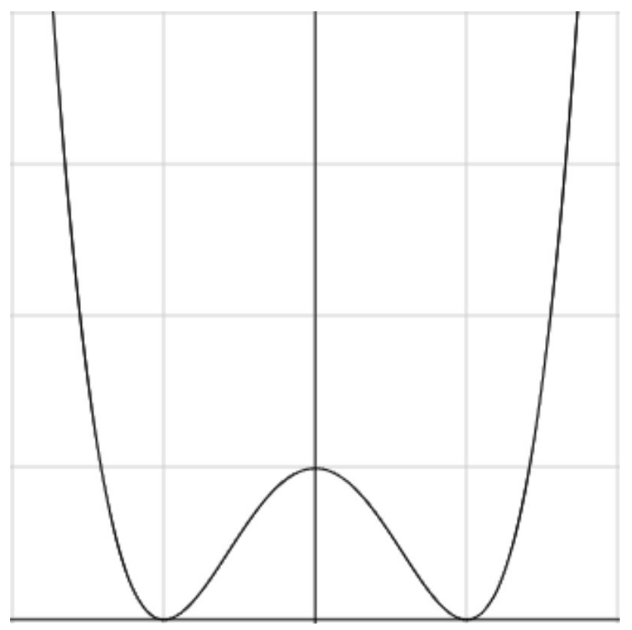
\includegraphics[scale=0.5]{higgsPotential.png}
   \caption{Higgs Potential where the y-axis has units of energy.}
   \label{fig:fig_1-8}
\end{figure}
In order to finish off our rules for creating Feynman diagrams we can draw the interaction vertex for the Higgs Boson in Figure \ref{fig:fig_1-9}. 
It can interact with any massive particle, including itself. 
The Higgs Boson has no charge, no spin and a mass of 126 $\frac{GeV}{c^2}$.

\begin{figure} %  figure placement: here, top, bottom, or page
   \centering
      \feynmandiagram[horizontal=a to b] {
         i1  [particle=massive particle] -- [fermion] a -- [fermion] i2  [particle=massive particle],
         a -- [scalar, edge label=Higgs] b, 
      };
   \caption{Higgs Boson Vertex.}
   \label{fig:fig_1-9}
\end{figure}
\clearpage
\section{What's Left?}

Now that we have a good understanding of the SM, what can we do with it? Well, to start, it isn't complete. 
Gravity is noticeably absent in the SM. This is possibly a little embarrassing for physics because gravity was the first fundamental force to be properly quantified when Newton wrote down his 3 laws.
Our current understanding of gravity, through the theory of General Relativity, does not mesh nicely with the equations of the SM. Large and complicated theoretical efforts have been working very hard to try to reconcile this difference but it still remains today. 
The discovery of a graviton, thought to be a spin-2 boson, would aid physicists greatly in completing our understanding of the fundamental forces of nature.

Beyond that, the visible matter in our universe only makes up about 4\% of the stuff in it. Physicists have good evidence that the universe is roughly 25\% matter so what is the other 21\%?
This extra stuff is theorized to be ``dark matter'', i.e. not interacting in a way we can directly detect, and is not currently included in the SM. There are many theories and experiments working on this question but no answer has come yet. Another problem is that we don't even fully understand the roughly 4\% of baryonic matter we do know about. The majority of this matter is made of particles but why? Why are there not more anti particles? It is not clear why there would be an asymmetry to the amount of matter vs anti matter. 
Some progress has been made recently on this question but the answer is still incomplete.

So given that we seem to be missing many answers to questions about known measurable physical phenomenon, how do we explain them? Theorists spend their days creating answers for these questions in a manner that would be consistent with the current SM.
These theories are know as ``Beyond Standard Model'' (BSM) and can address one or all of the known issues with the SM. Now we shall talk about a few BSM theories that will be relevant to this experiment.
%\printbibliography[title=References]}
%\end{refsection}
%
%\begin{refsection}[myrefs.bib]
\chapter{Beyond the Standard Model}
\label{chap:two}
In the last chapter we discussed the major parts of the SM, detailed some of the rules for working with it, and then talked briefly about what has been left out.
The SM itself actually imposes many constraints, so any BSM theory must conform to those constraints. It should also be pointed out that there have been many searches, but very little evidence, of BSM physics.
This does not exclude BSM physics, it just creates another set of constraints that must be satisfied along with the constraints already set by the SM. One of the most pressing questions about the SM, and one of the most relevant for the following experiment, is called the hierarchy problem.

\section{The Hierarchy Problem}

To understand the hierarchy problem, we need to revisit the Higgs boson feynman diagrams. If you recall, we can build up diagrams by adding vertices together. This then is a valid diagram between 4 particles that is mediated by a Higgs boson:
\begin{figure} %  figure placement: here, top, bottom, or page
    \centering
       \feynmandiagram[horizontal=a to b] {
          i1  [particle=1] -- [fermion] a -- [fermion] i2  [particle=2],
          a -- [scalar, edge label=Higgs] b, 

          f1  [particle=3] -- [fermion] b -- [fermion] f2  [particle=4],
       };
    \caption{A tree level Higgs diagram}
    \label{fig:fig_2-1}
 \end{figure}

Figure \ref{fig:fig_2-1} is what we call a ``tree level'' diagram. We can add possible interactions in the middle of the tree diagram creating what are called ``loops'', like in figure \ref{fig:fig_2-2}.

\begin{figure} %  figure placement: here, top, bottom, or page
    \centering
       \feynmandiagram[horizontal=b to c] {
          i1  [particle=1] -- [fermion] a -- [fermion] i2  [particle=2],
          a -- [scalar] b,
          b -- [fermion,half left,looseness=1.5] c-- [fermion,half left,looseness=1.5] b,  
          c -- [scalar] d,
          f1  [particle=3] -- [fermion] d -- [fermion] f2  [particle=4],
       };
    \caption{A loop level Higgs diagram}
    \label{fig:fig_2-2}
 \end{figure}

Since all we do is measure the incoming and outgoing particles, we do not know which of the diagrams is physically happening. 
The SM starts with what we call a ``bare'' mass term, in this case $m_H^{bare}$, and then when adding loops\footnote{This process of adding loops can create some wacky looking diagrams. However, even wacky diagrams can be experimentally relevant.}, it makes quantum corrections to the bare mass.
So, the mass we measure is actually:
\begin{equation}
    m_H = m_H^{bare} \times ( 1 + \sum_{\text{all loops}} \text{quantum loop corrections} ) 
    \label{eq:eq_bareMH}
\end{equation}
The Higgs boson is a scalar, which for our purposes, means that when adding up the corrective terms, they do not start cancelling each other out in a well controlled manner.
Since we do measure a consistent Higgs mass, theoretically it is not satisfactory that we cannot predict this mass in the SM due to the lack of control of the quantum correction terms.
The reason that this is a problem is that in the theoretical calculations of these quantum corrections, the Higgs mass is quadratically sensitive to any scale that you introduce to the theory.
Energy scales are introduced to quantum corrections in order to carry out a process called renormalization. Simply stated, renormalization is the process by which we can remove any non-physical values, i.e infinities, that show up in our calculations.
This happens frequently when calculating quantum corrections so if when we try to renormalize our quantum corrections but the terms only grow in relative size, there will be a problem when we try to take a large sum of ALL possible corrections to the Higgs bare mass.
In this case, the infinities that we tried to regulate will show up all over again. Again, since we can measure the Higgs mass, and it is definitely NOT infinity, we need to find a way to control these quantum corrections, which is where BSM physics comes in.
\section{Possible Solutions to the Hierarchy Problem}

There are several theoretical models that propose solutions that solve the hierarchy problem. We will not detail all of these proposals, as that would take a thesis of its own. 
Here we will give an overview of the two solutions that are most relevant to our experiment. They are Warped Extra Dimensions (WED) and Minimal Supersymmetric extensions to the SM (MSSM).

\subsection{Warped Extra Dimensions}

In classical physics, the notions of space and time are fixed to 4 dimensions, 3 space and 1 time.
In quantum physics, there is no a priori reason we cannot consider additions to the amount of spacetime dimensions.
After Einstein's newly introduced theory of 4-D spacetime, the General Theory of Relativity, researchers started asking if it was possible that what we see as 4-D spacetime is really 5-D, where the 5th dimension is compactified or warped in some way as to avoid easy detection.
The first of these theories is called Kaluza-Klein Theory and was originally published by Kaluza in 1921. This theory was originally unused as it did not offer many testable predictions. However, there have been many improvements in recent decades.

One of the recent improvements, indeed the one that is most experimentally relevant to us, is WED. 
The WED models have an extra spatial dimension compactified between two branes, with the region between (called the bulk) warped via an exponential metric ${\kappa l}$, $\kappa$ being the warp factor and $l$ the coordinate of the extra spatial dimension~\cite{Giudice:2000av}. 
For our purposes, we can think of branes as the ``boundaries'' to the spacetime in which we live. They are lower dimensional spaces that are dynamic and can effect the fields that propagate the forces we see in nature.
In these WED models, we can think of the ``low energy'' versions of our theories, i.e. the SM, as ``living'' on one brane. Here living on a brane means that the fields in the field theory do not propagate into all of the available spatial dimensions, in this case the bulk.
Then the ``high energy'' versions will live on the other and the bulk will mediate between them. The original version of these theories had only gravity propagating in the bulk, but that it is not the only thing that may propagate in the bulk of a WED theory \footnote{Other particles, namely SM fermions and bosons can propagate in the bulk.}.
In the literature, the ``low energy'' brane is called the infrared (IR) brane and the ``high energy'' brane is called the ultraviolet (UV) brane. 
These two scales, UV and IR, are very important for theoretical discussions of the behavior of SM theories. Since we will not delve into those details, I described what they are for your future reference.

In WED models, there can exist excitations, which is the mathematical way we think of particles in their respective fields, that are of the type described in Kaluza-Klein theory, so called KK excitations, and which propagate in the bulk.
The prediction from WED is that these excitations will be spin-2 bosons called KK gravitons. These would mediate gravity in the bulk and be a way to incorporate gravity into the SM. 
They also predict spin-0 particles, called radions, which are scalar versions of gravitons. 
These KK gravitons and radions are predicted to interact with the weak force which in turn allows them to interact with the SM Higgs boson and give them mass.

The radion serves another purpose. One question you might have thought to ask is, what is the size of the extra dimension that you keep talking about? 
If it is so small that we do not detect it, then how small is small enough to be undetectable? 
This is not currently known, however, the radion is produced from spontaneous symmetry breaking and therefore, takes a VEV.
This radion VEV then sets the scale of the size of the extra dimension or bulk that is between the UV and IR branes. 

\subsection{Minimal Supersymmetry}

Another way we can attempt to solve the hierarchy problem is to introduce a new class of theories called Supersymmetry.
In supersymmetric theories, each particle has a superpartner particle that is different from the anti-particle.
These extra particles would add cancelling terms to the equation in \ref{eq:eq_bareMH} which would allow the quantum correction terms to be controlled.
There are many supersymmetric models, each with small differences to account for the issues seen in the SM. We will not be able to cover all of the known supersymmetry models and will focus on the MSSM models.

MSSM models make what is called the ``minimal'' extension to the standard model. These minimal extensions take each SM fermion and add a superpartner, known as a sfermion (squarks or sleptions).
They also take each gauge field \footnote{A gauge field is the mathematical mechanism behind the SM forces. I do not introduce the machinery because it is quite extensive and would be a thesis in itself.} and add a gaugino, which is a propagating fermion for the field.
While this sounds overly simplistic, it adds its own version of complications after solving the hierarchy problem. 
For example, if these so called superpartners are just different version of their respective particles, and with the same mass, then we should have discovered them long ago.
Since we haven't, we must assume that there is a mass scale above which all of these superpartners live. 

Again, there are several ways to accomplish this addition of mass. 
However, they all involve a form of spontaneous symmetry breaking, recall how the Higgs field picks up a VEV, of the supersymmetry that generates all of these new particles.
This symmetry breaking is the underlying cause of the masses that these superpartners have. This is also very similar to the case of the electroweak interaction. 
In both of these cases, in the UV limit of these theories, the symmetry is preserved. As soon as we move from the UV to the IR, the symmatry is broken. 
The mathematical details here are not necessary for this thesis, so we will skip them. They also contain colloquial language that can be very confusing \footnote{For example, those of you who are theory inclined will recall that Goldstone bosons exist whenever a field breaks a symmetry and generates a VEV. When we promote that symmetry to a gauge symmetry, for some reason it is fashionable to say that the Goldstone boson is ``eaten'', which I found very confusing initially since it implies that the boson disappears instead transforming into the longitudinal polarization for the corresponding gauge field.}. 

\section{Predictions of WED and MSSM}
In the standard model (SM), the pair production of Higgs bosons ($\PH$)~\cite{HiggsDiscoveryAtlas,HiggsDiscoveryCMS,CMSHiggsLongPaper} in proton-proton ($\Pp\Pp$) collisions at $\sqrt{s} = 13\TeV$ is a rare process~\cite{deFlorian:2013jea}.
However, the existence of massive resonances decaying to Higgs boson pairs ($\PH\PH$) in many new physics models may enhance this rate to observable levels, even with current experimental data.
For instance, WED models~\cite{Randall:1999ee} contain new particles such as the spin-0 radion~\cite{Goldberger:1999uk,Csaki:1999mp,Csaki:2000zn} and the spin-2 first KK excitation of the graviton~\cite{Davoudiasl:1999jd,DeWolfe:1999cp, Agashe:2007zd}, which have sizable branching fractions to $\PH\PH$.

In WED models, the reduced Planck scale ($\overline{\Mpl} \equiv \Mpl/8\pi$, \Mpl being the Planck scale) is considered a fundamental scale.
The free parameters of the model are $\kappa / \overline{\Mpl}$ and the UV cutoff of the theory $\LambdaR \equiv \sqrt{6} \re^{-\kappa l} \overline{\Mpl}$~\cite{Goldberger:1999uk}.
In $\Pp\Pp$ collisions, the graviton and the radion are produced primarily through gluon-gluon fusion and are predicted to decay to $\PH\PH$~\cite{Oliveira:2014kla}.

Other scenarios, such as the two-Higgs doublet models~\cite{Branco:2011iw} (in particular, the minimal supersymmetric model~\cite{Djouadi:2005gj}) and the Georgi-Machacek model~\cite{GEORGI1985463} predict spin-0 resonances that are produced primarily through gluon-gluon fusion, and decay to an $\PH\PH$ pair.
These particles have the same Lorentz structure and effective couplings to the gluons and, for narrow widths, result in the same kinematic distributions as those for the bulk radion.

% Searches for a new particle $\PX$ in the $\PH\PH$ decay channel have been performed by the
% ATLAS~\cite{Aad:2014yja, Aad:2015uka, Aad:2015xja} and
% CMS~\cite{Khachatryan:2014jya, Khachatryan:2015year, Khachatryan:2015tha,Khachatryan:2016sey,Khachatryan:2016cfa}
% Collaborations in $\Pp\Pp$ collisions at $\sqrt{s} =  7$ and 8\TeV.
% More recently, the ATLAS Collaboration has published limits on the production of a KK bulk graviton, decaying to $\PH\PH$, in the $\bbbar\bbbar$ final state, using $\Pp\Pp$ collision data at $\sqrt{s} = 13\TeV$, corresponding to an integrated luminosity of 3.2\fbinv~\cite{Aaboud:2016xco}. Because the longitudinal components of the $\PW$ and $\PZ$ bosons couple to the Higgs field in the SM, a resonance decaying to $\PH\PH$ potentially also decays into $\PW\PW$ and $\PZ\PZ$, with a comparable branching fraction for $\PX\to\PZ\PZ$, and with a branching fraction for $\PX\to\PW\PW$ that is twice as large.
% Searches for $\PX \to \PW\PW$ and $\PZ\PZ$ have been performed by ATLAS and CMS~\cite{ATLASVV,ATLASWV,ATLASZV,Khachatryan:2014hpa,CMSZVWV,ATLAS13TeV_WW_WZ_ZZ_allhad,ATLAS13TeV_WW_WZ_semilep}.

% This analysis note reports on the search for a massive resonance decaying to an $\PH\PH$ pair, in the $\bbbar\bbbar$ final state (with a branching fraction $\approx$33\%~\cite{deFlorian:2016spz}), performed using a data set corresponding to \intLumi of $\Pp\Pp$ collisions at $\sqrt{s} = 13\TeV$.
% This search significantly improves upon the CMS analyses performed using the LHC data collected at $\sqrt{s} = 13$ in 2016~\cite{B2G-16-026-paper,B2G-17-019-paper}.
%\printbibliography[title={References}]
%\end{refsection}
%
%\begin{refsection}[myrefs.bib]
\chapter{How to find Pairs of Boosted Higgs Bosons (The CMS Detector at CERN)}
\label{chap:three}

% Introduction
\sect{\lipsum*[20][1]}

\subsect{\lipsum*[20][2]}

\lipsum[1-3]

\subsect{\lipsum*[20][3]}

\lipsum[4-5]

\subsect{\lipsum*[20][4]}

\lipsum[7-8]

\subsect{\lipsum*[20][5]}

\lipsum[10-12]

% Figure 3-1
\begin{figure}[tb]
   \centering
%   
\includegraphics[width=\textwidth,height=\textheight,keepaspectratio]{fig_3-1}
   
\includegraphics[scale=1]{fig_3-1}
   \caption[{\lipsum*[31][1]}]{\lipsum*[31][1-5]}
   \label{fig:fig_3-1}
\end{figure}

% Materials and Methods
\sect{\lipsum*[21][1]}

\subsect{\lipsum*[21][2]}

\lipsum[13]

\subsect{\lipsum*[21][3]}

\lipsum[14-15]

\subsect{\lipsum*[21][4]}

\lipsum[16-17]

\subsect{\lipsum*[21][5]}

\lipsum[18]

\subsect{\lipsum*[21][6]}

\lipsum[19-20]

\subsect{\lipsum*[21][7]}

\lipsum[21]

\subsect{\lipsum*[21][8]}

\lipsum[22]

\subsect{\lipsum*[21][9]}

\lipsum[23-24]

\subsect{\lipsum*[21][10]}

\lipsum[25-26]

\subsect{\lipsum*[21][11]}

\lipsum[27-28]

\subsect{\lipsum*[21][12]}

\lipsum[29-30]

\subsect{\lipsum*[21][13]}

\lipsum[31]

% Results
\sect{\lipsum*[22][1]}

\subsect{\lipsum*[22][2]}

\lipsum[27-32]

% Figure 3-2
\begin{figure}[p]
   \centering
%   
\includegraphics[width=\textwidth,height=\textheight,keepaspectratio]{fig_3-2}
   
\includegraphics[scale=1]{fig_3-2}
   \caption[{\lipsum*[32][1]}]{\lipsum*[32][1-5]}
   \label{fig:fig_3-2}
\end{figure}

\subsect{\lipsum*[22][3]}

\lipsum[33-35]

% Figure 3-3
\begin{figure}[p]
   \centering
%   
\includegraphics[width=\textwidth,height=\textheight,keepaspectratio]{fig_3-3}
   
\includegraphics[scale=1]{fig_3-3}
   \caption[{\lipsum*[33][1]}]{\lipsum*[33][1-5]}
   \label{fig:fig_3-3}
\end{figure}

\subsect{\lipsum*[22][4]}

\lipsum[36-37]

% Figure 3-4
\begin{SCfigure}[\sidecaptionrelwidth][p]
   \centering
%   
\includegraphics[width=\textwidth,height=\textheight,keepaspectratio]{fig_3-4}
   
\includegraphics[scale=0.90]{fig_3-4}
   \caption[{\lipsum*[34][1]}]{\lipsum*[34][1-5]}
   \label{fig:fig_3-4}
\end{SCfigure}

\subsect{\lipsum*[22][5]}

\lipsum[38-40]

% Figure 3-5
\begin{figure}[p]
   \centering
%   
\includegraphics[width=\textwidth,height=\textheight,keepaspectratio]{fig_3-5}
   
\includegraphics[scale=1]{fig_3-5}
   \caption[{\lipsum*[35][1]}]{\lipsum*[35][1-5]}
   \label{fig:fig_3-5}
\end{figure}

\subsect{\lipsum*[22][6]}

\lipsum[41-43]

% Figure 3-6
\begin{figure}[p]
   \centering
%   
\includegraphics[width=\textwidth,height=\textheight,keepaspectratio]{fig_3-6}
   
\includegraphics[scale=1]{fig_3-6}
   \caption[{\lipsum*[36][1]}]{\lipsum*[36][1-2]}
   \label{fig:fig_3-6}
\end{figure}

% Discussion
\sect{\lipsum*[22][7]}

\lipsum[44-51]

% Figure 3-7
\begin{figure}[p]
   \centering
%   
\includegraphics[width=\textwidth,height=\textheight,keepaspectratio]{fig_3-7}
   
\includegraphics[scale=1]{fig_3-7}
   \caption[{\lipsum*[37][1]}]{\lipsum*[37][1-2]}
   \label{fig:fig_3-7}
\end{figure}

% Figure 3-8
\begin{figure}[p]
   \centering
%   
\includegraphics[width=\textwidth,height=\textheight,keepaspectratio]{fig_3-8}
   
\includegraphics[scale=1]{fig_3-8}
   \caption[{\lipsum*[38][1]}]{\lipsum*[38][1-2]}
   \label{fig:fig_3-8}
\end{figure}

% Figure 3-9
\begin{figure}[p]
   \centering
%   
\includegraphics[width=\textwidth,height=\textheight,keepaspectratio]{fig_3-9}
   
\includegraphics[scale=1]{fig_3-9}
   \caption[{\lipsum*[39][1]}]{\lipsum*[39][1-2]}
   \label{fig:fig_3-9}
\end{figure}

% Figure 3-10
\begin{figure}[p]
   \centering
%   
\includegraphics[width=\textwidth,height=\textheight,keepaspectratio]{fig_3-10}
   
\includegraphics[scale=1]{fig_3-10}
   \caption[{\lipsum*[40][1]}]{\lipsum*[40][1-2]}
   \label{fig:fig_3-10}
\end{figure}

%\printbibliography[title={References}]
%\end{refsection}
%
%\begin{refsection}[myrefs.bib]
\chapter{Algorithms that Detect Interesting Higgs Boson Candidates}
\label{chap:four}
The analysis we perform will be looking for 2 Higgs bosons which decay into 4 total b quarks.
The 4b final state will decay into jets. 
Jets resulting from pairs of b quarks are identifiable because the parent Higgs jets are identifiable with a high degree of accuracy.
The following sections will detail how this is accomplished.
\section{Soft-Drop Mass Algorithm}

As previously stated, the decay signature of the Higgs boson we are looking for is a pair of b quarks.
When heavy particles, like the Higgs boson, decay to a pair of quarks, the angle between those two quarks is dependant only on the velocity of the parent heavy particle\footnote{This is for the lab frame. In the rest frame of the parent particle the two quarks will decay back to back.}.
Low energy Higgs will produced two distinct b quark jets where high energy Higgs will produce a collimated, also called ``boosted'', single jet.
Since we then are concerned with the energy of the parent particle, it is important for us to accurately determine if we are looking at the parent particle or not.
If you recall, pileup causes jets from background processes to appear to have the same mass\footnote{We will sometimes substitute mass and energy freely since the lorentz invariant mass is also useful to measure as a proxy for energy.} as a jet from a heavier particle.
Of the grooming algorithms that exist to differentiate these two cases, we will use the \textit{Soft-Drop Mass Algorithm}.

The algorithm starts by unclustering the jet, recall we cluster jet with the Anti-$k_T$ algorithm, and then categorizing the constituents as pseudo-jets.
These pesudo-jets are then compared to each other using the formula:
\begin{equation}
    \frac{min(p_{T,1},p_{T,2})}{p_{T,1}+p_{T,3}} > z
\end{equation}
where $z$ determines the strength of the cut. Our analysis uses $z = 0.1$\textbf{CHECK THIS} as the cut. 
If this condition is true, then the jet is kept. Otherwise, it is thrown out for consideration as a heavy particle jet.
This helps mimic the conditions that a real heavy particle would cause rather than those that come from pileup.
Since we use this as a discriminator for heavy particle jets and their decays, we will use it as a tagging variable in our analysis.

\section{Deep AK8 Mass Decorrelated Tagger}

Anotehr way to tag Higgs bosons is through exploiting the information that is gained when creating particle flow candidates and using a machine learning algorithm to identify hadronically decaying heavy particles, like the Higgs boson.
The algorithm also further delineates the decay product into decay modes, i.e. a Higgs to two b quarks. This algorithm is called \textit{Deep-AK8}.
The algorithm begins by defining two lists of inputs. The first list is a list of 100\footnote{Typically, jets do not have more than 100 constituent particles so using this cap contributes to a negligible loss of information.} jet constituent particles list in decreasing $p_T$.
Measured properties of each particle, $p_T$, the energy deposit, the charge, the angular separation between the particle and the
jet axis, etc., are used to help the algorithm extract features related to the substructure of the jet.
Charged particle will also have information from tracking including track quality and displacement.
These features are especially useful for identifying heavy flavour quarks, like the b quark. In total there are 42 pieces of information for each particle in the list.

The second list is comprised of secondary vertex information. Recall that the primary vertex relates to the location of the initial proton-proton collision.
The secondary vertex relates to the location of the next decay. So then this can be useful for identifying decaying products.
Notably, the b quark has a longer lifetime than other quarks, so its decay vertex, the secondary vertex, is very useful in its identification. This is shown pictorially in Figure \ref{fig:fig_4-1}.
This list will contain up to 7 secondary vertices as well as kinematic information about the vertices, displacement, and quality of the vertices.
Since this is a large amount of information, it poses a challenge to directly using it. The correlation between these inputs is very important for identifying particles so a custom neural network architecture is used.

\begin{figure} %  figure placement: here, top, bottom, or page
    \centering
 %   
\includegraphics[width=\textwidth,height=\textheight,keepaspectratio]{fig_2-1}
    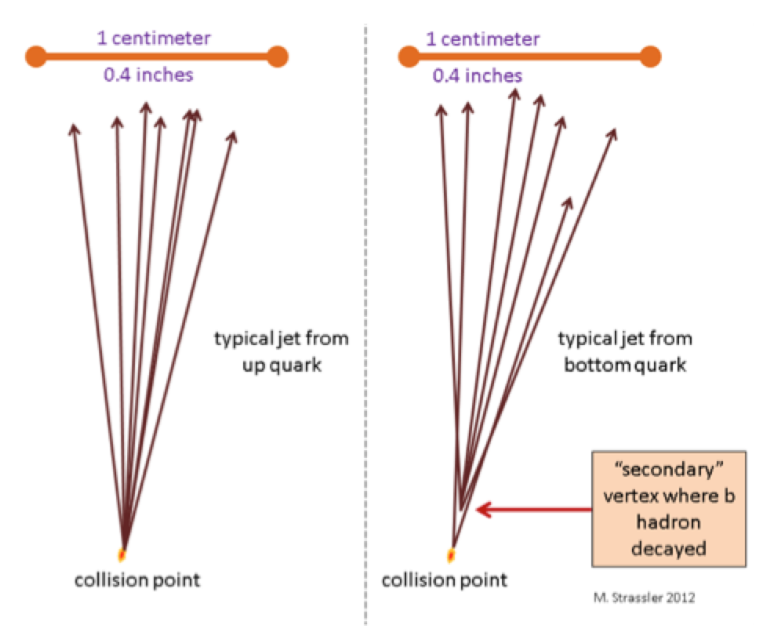
\includegraphics[scale=0.5]{bquarkSV.png}
    \caption{A diagram of how quarks behave in the detector.}
    \label{fig:fig_4-1}
 \end{figure}
\subsection{Custom Neural Network}

A custom deep neural network (DNN) is constructed in order to handle the complicated correlations between inputs.
This consists of two steps. The first step is to apply a convolutional neural network (CNN) is used to process each of the two lists in parallel.
Then in the second step, the output of the CNN is combined by a simple, fully connected network to perform the classification of the jet.
A re-weighting is used avoid any dependance on jet $p_T$ that can occur when training the network with a mix of background and signal samples.
The network architecture is shown in Figure \ref{fig:fig_4-2}.
\begin{figure} %  figure placement: here, top, bottom, or page
    \centering
 %   
\includegraphics[width=\textwidth,height=\textheight,keepaspectratio]{fig_2-1}
    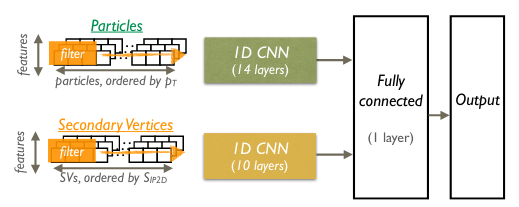
\includegraphics[scale=0.7]{deepAK8Arch.png}
    \caption{A diagram of the network architecture of the DeepAK8 Algorithm.}
    \label{fig:fig_4-2}
 \end{figure}
\subsection{Custom Neural Network}
If one wants to use mass as a discriminating variable, then a mass-decorrelated version of the DeepAK8 algorithm is used.
This will add a feature to the network architecture that acts as a mass prediction score. This score then acts as a penalty weight to prevent the network from extracting features that correlate with mass.
This allows the algorithm to become largely mass independent. This will decrease the power of the algorithm. The network architecture is shown in Figure \ref{fig:fig_4-3}.
The training of the DeepAK8-MD tagger was conducted on jets with a softdrop mass ($m_{SD})$ between 30 and 250 $GeV$ so any jet outside of that range should not be used in conjunction with this algorithm.
\begin{figure} %  figure placement: here, top, bottom, or page
    \centering
 %   
\includegraphics[width=\textwidth,height=\textheight,keepaspectratio]{fig_2-1}
    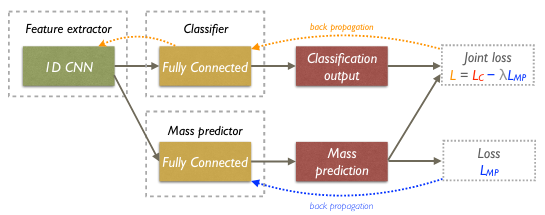
\includegraphics[scale=0.7]{deepAK8MDArch.png}
    \caption{A diagram of the network architecture for the Mass-Decorrelated version of the DeepAK8 Algorithm.}
    \label{fig:fig_4-3}
 \end{figure}

\subsection{Advantages}

A similar analysis to the one performed in this analysis was completed with a different tagging algorithm and on only the 2016 data.
This ``Double B'' tagger worked by using a boosted decision tree learning algorithm to assign a score to the jet measuring the likelihood that it contains two b quarks.
It is also mass and $p_T$ independent. At the time of that analysis, it was the best performing tagger available. However, it had drawbacks.
The biggest drawback is that, while it attempted to use jet substructure information, it needed to be supplemented with directly measured substructure variables.
The penalty is paid in the systematic uncertainty of those variables, which unfortunately is relatively high.
The DeepAK8 tagger uses those substructure variables more efficiently so we can actually drop them as an extra discriminator and avoid paying the same penalty.

\section{Deep Jet Tagger}

The Deep Jet algorithm is used to find jets that are not pairs of b quarks but individual b quarks, i.e AK4 jets. 
It uses a similar two network structure like the DeepAK8 algorithm but substitutes a recurrent neural network (RNN) instead of using the simple fully connected network that DeepAK8 uses.
It starts by training the CNN on separate collections of charged and neutral jet particle flow candidates. 
The outputs are then fed into the RNN. After that training, the resultant output is combined with variables such as $p_T$ and $\eta$ of each jet and then processed by a dense layer with 7 hidden layers.
The network architecture is shown in Figure \ref{fig:fig_4-4}
A score is then given based on the likelihood of the decay product being a heavy flavour quark. The improvement over the algorithm previously used to identify AK4 jets, called Deep CSV, is gained by using a larger set of inputs and a better neural network model.
\begin{figure} %  figure placement: here, top, bottom, or page
    \centering
 %   
\includegraphics[width=\textwidth,height=\textheight,keepaspectratio]{fig_2-1}
    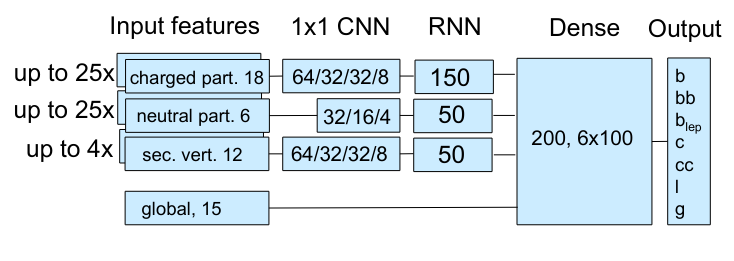
\includegraphics[scale=0.5]{deepJetArch.png}
    \caption{A diagram of the network architecture for the Deep Jet Algorithm.}
    \label{fig:fig_4-4}
 \end{figure}

%\printbibliography[title={References}]
%\end{refsection}
%
%\begin{refsection}[myrefs.bib]
\chapter{HH4b: Event Selection}
\label{chap:five}

In this search, the $\PX \to \PH\PH$ decay of a very heavy new resonance X would result in two highly Lorentz-boosted Higgs bosons.  Due to its large Lorentz boost, at least one of the decay products of each $H \to b\bar b$ decay are collimated, and reconstructed within a single AK8 jet. 
These are reconstructed using jet substructure and jet flavour-tagging techniques ~\cite{Butterworth:2008iy,Cooper:2013kia,Gouzevitch:2013qca} and, once they pass this selection, referred to as $\PH$ jets.

The standard model background consists mostly of multijet events, and is estimated using several control regions defined in the phase space of the masses and flavour-tagging discriminators of the two $\PH$ jets, and the $\PH\PH$ dijet invariant mass, allowing the background to be predicted over the entire $\mx$ range. 
The final event selection also contains a smaller amount of $t\bar{t}$+jets, which is modeled by 2D templates from the simulation; these templates are allowed to morph within uncertainties, and this morphing is governed by a number of nuisance parameters.
The dijet $M_{jj}$ mass distribution of the two leading Higgs-tagged jets corresponds to the invariant mass of the resonance searched for. 

The effectiveness of constraining the mass of each Higgs candidate to a $M_H$ window ~\cite{CMS-PAS-B2G-16-026} has been studied extensively. This technique was validated in the resolved and boosted searches~\cite{CMS-PAS-B2G-16-026}. One needs a variable which `corrects' the dijet invariant mass by the amount by which the individual H-jet masses are above or below the mass of the Higgs boson.  This approach is similar to a mass constraint in a $\chi^2$ fit but it does not bias the H-jet mass distribution. Therefore, the variable:
\begin{equation}
M^{red}_{jj} = M_{jj} - (M^1_{jet} - M_H) - (M^2_{jet} - M_H) \label{eq:mred}
\end{equation} 
is used to provide the best resolution of $M_{jj}$. 

The signal would appear as a peak in the $M_{jj}$ spectrum on top of a smooth background distribution. With this in mind, our analysis strategy is as follows:
\begin{itemize}
\item The signal region has two H tagged jets
\item We will be using the reduced mass, defined in Equation \ref{eq:mred}:
\item The main backgrounds are (i) QCD and (ii) $t\bar{t}$.  Their ratio depends on the H-tagger used (double-b or Deep AK8).
\item $t\bar t$+jets  is obtained from template-morphed MC shapes ($t\bar{t}$the nuisances are constrained in the fit to data)
\item QCD is obtained from H mass sidebands, and a ratio of pass and fail events, which is a smooth analytical function of $m_H$ and $m_{reduced}$ ($R_{p/f}$) (w.r.t. H-tag). This is accomplished by assigning one AK8 jet to pass the H-tagging first, and be `preselection side', and the other one is used in the 2DAlphabet background estimate and is called `Alphabet side'. 
\item Then an Alphabet style procedure is run in order to estimate the background and provide the $R_{p/f}$. The passing distribution in the signal region is modeled inside Combine by multiplying the failing distribution in data by the $R_{p/f}$.
\end{itemize}
%\newpage

\section{Event Selection\label{sec:EvtSel}}
\subsection{Fully Merged Topology}
Events passing the baseline triggers are further required to pass selection criteria close to the signal selection in the actual analysis:
\begin{itemize}
\item Leading two AK8 jets in the event with $\pt > 300 GeV$ and $|\eta| < 2.4$;
\item $\Delta \eta_{jj} < 1.3$ for the leading two AK8 jets, where $\Delta \eta_{jj} = |\eta_{1stFatJet} - \eta_{2ndFatJet}|$.
\end{itemize}
The details of these variables and selections are later described in Sections ~\ref{ss:JetSel} and ~\ref{ss:EvtSelMass}. 

For the $\Delta \eta_{jj}$ cut, the rationale is to suppress QCD, since the production of a heavy $X \to HH$ will be mostly central (as the bulk of the energy of the incoming partons would be used to create X), and thus the X will usually have low boost along the z axis. In contrast, in QCD, the valence quarks that glance off of each other and each go at very high eta to produce very large dijet invariant mass events. So this cut is a natural way to suppress QCD for very high masses of X. Events are required to have at least two jets, of which the two leading jets each need to have $\pt > 300 GeV$ and pseudorapidity $|\eta| < 2.4$. These two jets also need to be relatively close, $\Delta \eta_{jj} < 1.3$ in order to reduce any contribution from multijet events. A detailed study of this is given in Appendix B of \cite{CMS-PAS-B2G-16-026}.

\subsection{Jet kinematics selection\label{ss:JetSel}}

Individual particles are reconstructed using a particle flow (PF) algorithm ~\cite{PFPAS2009,CMS-PAS-PFT-10-001}, that combines the information from all the CMS detector components. Each such particle is referred to as a PF candidate. The five classes of PF candidates are muons, electrons, photons, and charged and neutral hadrons. \\

The anti-$k_t$ algorithm \cite{antiKtAlgorithm}, implemented in FASTJET \cite{Cacciari:2011ma}, clusters PF candidates ~\cite{PFPAS2009,CMS-PAS-PFT-10-001} into jets using a distance parameter $R = 0.8$ (referred to as AK8 jets). In order to mitigate the the effect of pileup on the different jet observables, we take advantage of the available pileup per particle identification (PUPPI) \cite{puppi}. This method uses the local shape information, event pileup properties, and tracking information together in order to compute a weight describing how pileup-like a particle is. 

The jet 4-momenta are corrected to account for the difference between expected and measured momentum at the particle level, using a standard CMS correction procedure described in \cite{CMS-PAS-JME-10-003}. We use the Jet Energy Correction (JEC) and Jet Energy Resolution (JER) corrections as implemented by the NanoAODtools JetMetUncertainties module \footnote{See here \url{https://github.com/cms-nanoAOD/nanoAOD-tools/tree/master/python/postprocessing/modules/jme}}.  All jets are further required to pass tight jet identification requirements provided by JetMET POG \footnote{\url{https://twiki.cern.ch/twiki/bin/view/CMS/JetMET}}.

Additionally, all events are required to pass all of the recommended \footnote{https://twiki.cern.ch/twiki/bin/viewauth/CMS/MissingETOptionalFiltersRun2\#Analysis\_Recommendations\_for\_ana} filters which account for, among other things, missing energy (MET).

\subsection{\texorpdfstring{\PH}{H} mass selection\label{ss:EvtSelMass}}

The masses of the two leading jets can be used to suppress the multijet and $\ttbar$ backgrounds. The jet-grooming algorithm called Soft Drop (cite) is used to remove the contributions from the underlying event (UE) activity and pileup, as well as remove soft and wide-angle radiation.  The jet grooming leaves the hard prongs from a H$\to b\bar b$ unaffected, whereas it strips away most of the soft radiation from a QCD shower.  As a result, the masses of QCD jets are pushed lower, whereas the jet masses from true Higgs jets are largely unchanged. The invariant mass, $M_{jj}$, is calculated. 
%A dedicated jet energy calibration correction is applied to the softdrop mass (cite). The correction is derived in two steps. First, a weight to account for $\pt$ dependence at the generator level (``gen correction'') is computed. Second, an additional weight is calculated to account for any $\pt$ and $\eta$ dependence between the reconstructed and generated softdrop mass (``reco correction'') after the ``gen correction'' has been applied. This difference between reconstructed and generated softdrop mass is a $5-10\%$ effect \cite{CMS-PAS-B2G-16-026}.

\subsection{Deep AK8 Mass De-correlated H Tagger\label{ss:deepAK8}}
In order to identify the two jets most likely to contain two b quarks, we use the deep AK8 mass decorrelated Hbb tagger, labeled \texttt{deep\_TagMDHbbvsQCD} \cite{CMS:2019gpd} in nanoAOD version 5. This tagger uses customized machine learning methods and what is called the ``DeepAK8'' algorithm using particle level information and secondary vertex information. Each is split into a separate ``set'' and a 1D CNN is applied to each set. The output of that is fed into a fully connected network to perform the jet classification. A mass prediction network is added for the version we are using because it is not desirable to use the ``DeepAK8'' algorithm when the mass distribution is used to discriminate between signal and background, as is in this analysis. Further details can be found in \cite{CMS:2019gpd}. 

We have made a $S/\sqrt{B}$ study in order to optimize the working points for this tagger, were we measure the data-to-MC efficiency SF ourselves. It should be noted that, in the optimization, the change in the H-jet selection affects also the `preselection' H-jet." At each signal MC mass point, $S/\sqrt{B}$ is calculated and the working points are chosen as the average over all the signal MC mass points. \footnote{In the previous analysis \cite{CMS-PAS-B2G-16-026}, $\tau_N$ was used to quantify the degree to which jet constituents could be arranged into N subjets. The ratio $\tau_{21} = \tau_2 / \tau_1$ was calculated for both jets and contributed a systematic uncertainty of $5-15\%$ \cite{CMS-PAS-B2G-16-026}. This requirement has been dropped for this analysis. We are using more modern taggers, \texttt{deepAK8MD\_HbbvsQCD} \cite{CMS:2019gpd} for example, which have the substructure information already included. Since this selection criteria is now redundant, we drop it and gain by reducing our systematic uncertainty. This study is documented in Appendix C.} We are using 0.9 as the tight working point and 0.8 as the loose working point\footnote{See the Appendix for previous studies on the working point.}.
We also show cutflow diagrams to illustrate the working point efficiencies for these points chosen. 
\begin{figure}[!htb]
	\centering
	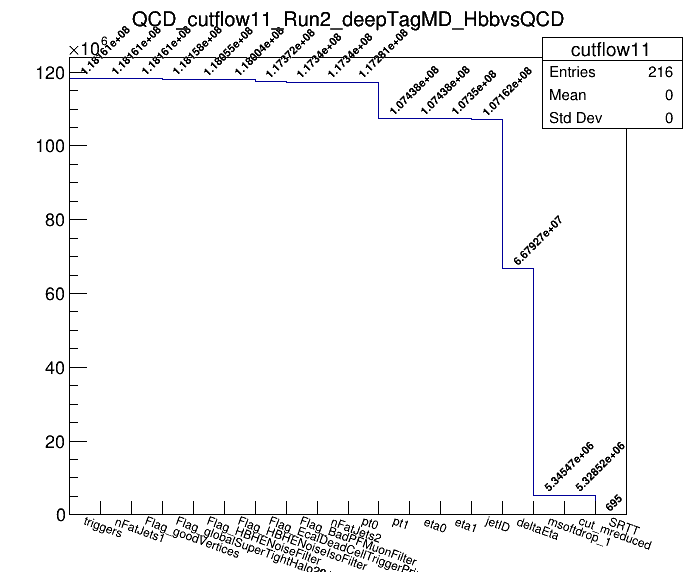
\includegraphics[width=0.8\textwidth]{Figures/QCD_cutflow11_Run2_deepTagMD_HbbvsQCD.png}
	\caption{Cutflow Diagram for Tight Tight QCD Selection}
	\label{fig:11CutflowqcdTT}
\end{figure}
\begin{figure}[!htb]
	\centering
	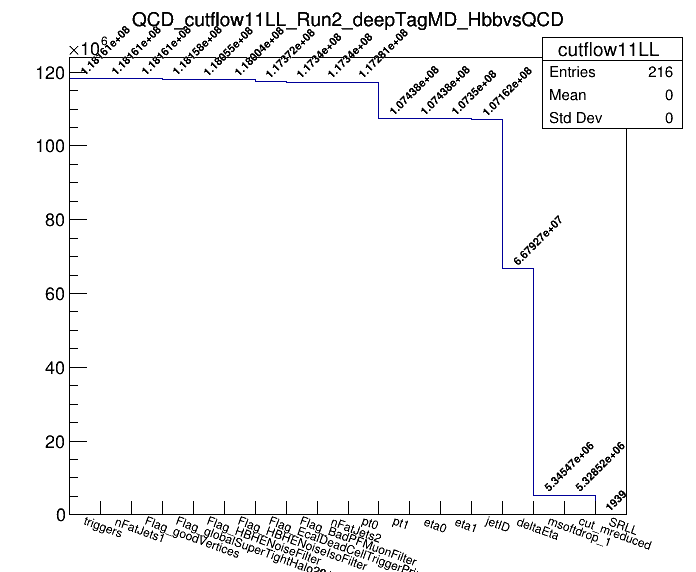
\includegraphics[width=0.8\textwidth]{Figures/QCD_cutflow11LL_Run2_deepTagMD_HbbvsQCD.png}
	\caption{Cutflow Diagram for Loose Loose QCD Selection}
	\label{fig:11CutflowqcdLL}
\end{figure}
\begin{figure}[!htb]
	\centering
    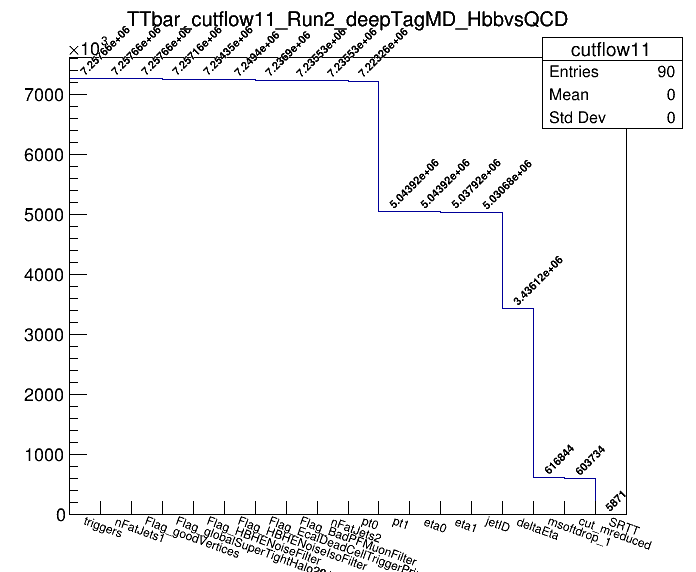
\includegraphics[width=0.8\textwidth]{Figures/ttbar_cutflow11_Run2_deepTagMD_HbbvsQCD.png}
	\caption{Cutflow Diagram for Tight Tight $\ttbar$ Selection}
	\label{fig:11CutflowttTT}
\end{figure}
\begin{figure}[!htb]
	\centering
    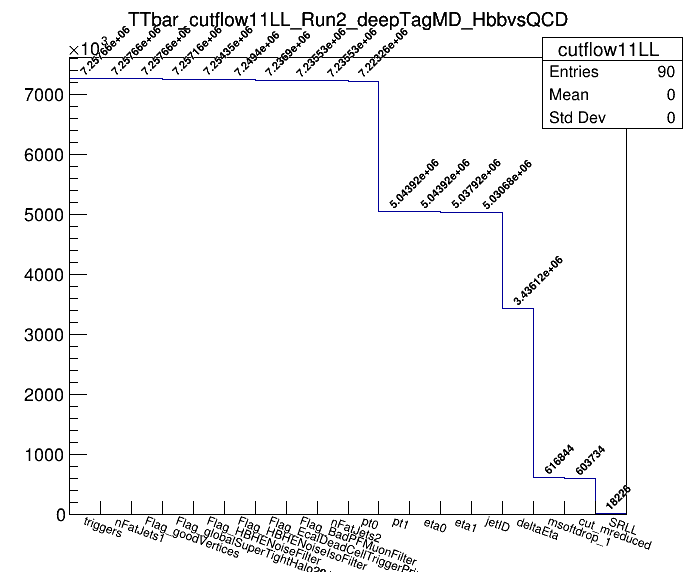
\includegraphics[width=0.8\textwidth]{Figures/ttbar_cutflow11LL_Run2_deepTagMD_HbbvsQCD.png}
	\caption{Cutflow Diagram for Loose Loose $\ttbar$ Selection}
	\label{fig:11CutflowttLL}
\end{figure}
\begin{figure}[!htb]
	\centering
    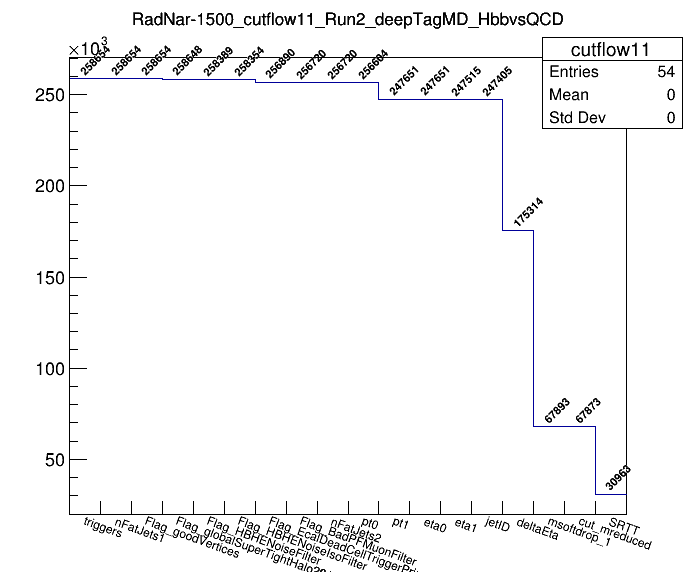
\includegraphics[width=0.8\textwidth]{Figures/radnar1500_cutflow11_Run2_deepTagMD_HbbvsQCD.png}
	\caption{Cutflow Diagram for Tight Tight Radion 1500 GeV Selection}
	\label{fig:11CutflowsigTT}
\end{figure}
\begin{figure}[!htb]
	\centering
    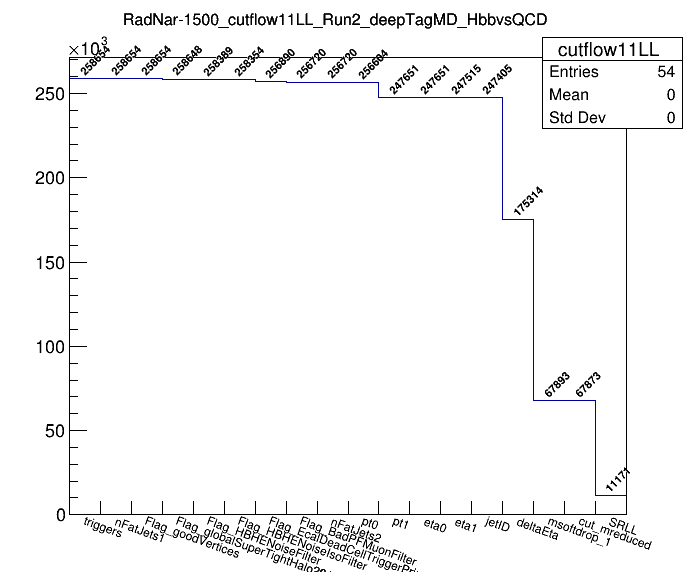
\includegraphics[width=0.8\textwidth]{Figures/radnar1500_cutflow11LL_Run2_deepTagMD_HbbvsQCD.png}
	\caption{Cutflow Diagram for Loose Loose Radion 1500 GeV Selection}
	\label{fig:11CutflowsigLL}
\end{figure}

% \begin{center}
% \begin{tabular}{ |c|c| } 
%  \hline
%  Background & Selection Efficiency \\ 
%  \hline
%  QCD & $> 99$\% \\ 
%  $\ttbar$ & $99.02$\% \\ 
%  RadNar-1500 & $54.38$\% \\   
%  \hline
% \end{tabular}
% \end{center}
\clearpage
\subsection{Boosted Event Selection\label{sec:EvtSel1p1}} 
The event selection follows the same as the trigger above but adding the following criteria:
\begin{itemize}
\item The soft drop mass of the two jets are $110 < M_{softdrop} < 140 GeV$, with all necessary jet mass corrections applied 
\item The dijet invariant mass, $M^{red}_{jj}$, $> 750$.
\end{itemize}
The soft drop mass window was optimized by making preliminary limits for three different windows. The results are shown in Figure \ref{fig:sdmasswindow} 
\begin{figure}[!htb]
	\centering
	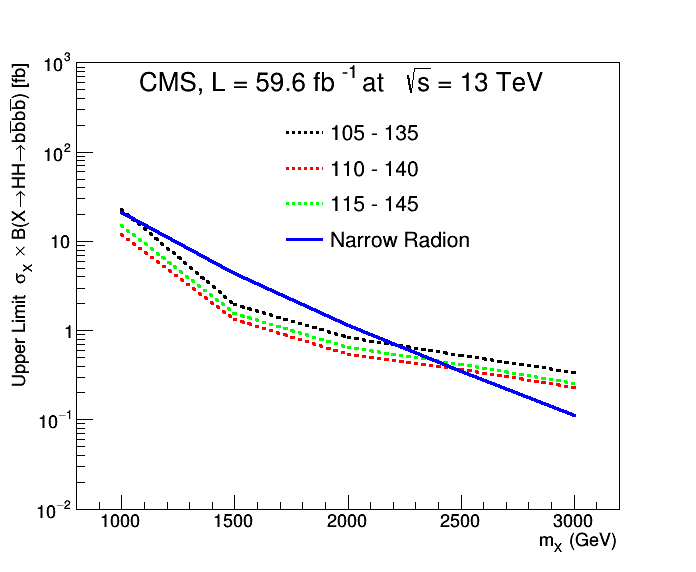
\includegraphics[width=0.8\textwidth]{Figures/limits_HH_combine_59.6fb_softdropwindow_limit_comparison_RadNar.png}
	\caption{Preliminary limits used to optimize the soft drop mass window.}
	\label{fig:sdmasswindow}
\end{figure}

\subsection{Identification of Higgs jets in boosted analysis\label{sec:EvtSelBoostedtagging}}
For the boosted analysis, events are required to pass the above selection criteria. The double b-tagger described in Section~\ref{ss:deepAK8} is used to identify the boosted Higgs jet in the boosted analysis. We then split the candidate events into tight-tight (TT) and loose-loose (LL) pass and fail regions. The algorithm to do this is as follows:
The 2D Alphabet method, with the signal region blinded, is then used to obtain the background estimate in the signal region. The possible combinations taken into account are:
\begin{itemize}
\item TT Pass: Both H-jets pass the tight operating point;
\item TT Fail: The leading H-jet fails the tight operating point and the subleading passes.
\item LL Pass: Both H-jets pass the loose working point but both fail the tight working point. This also means that if one jet passes the loose working point and the other passes the tight working point, the event will be classified as LL.
\item LL Fail: The leasing H-jet fails the loose operating point and the subleading passes the loose operating point. The subleading H-jet must also fail the tight working point.
\end{itemize}
\begin{figure}[!htb]
	\centering
	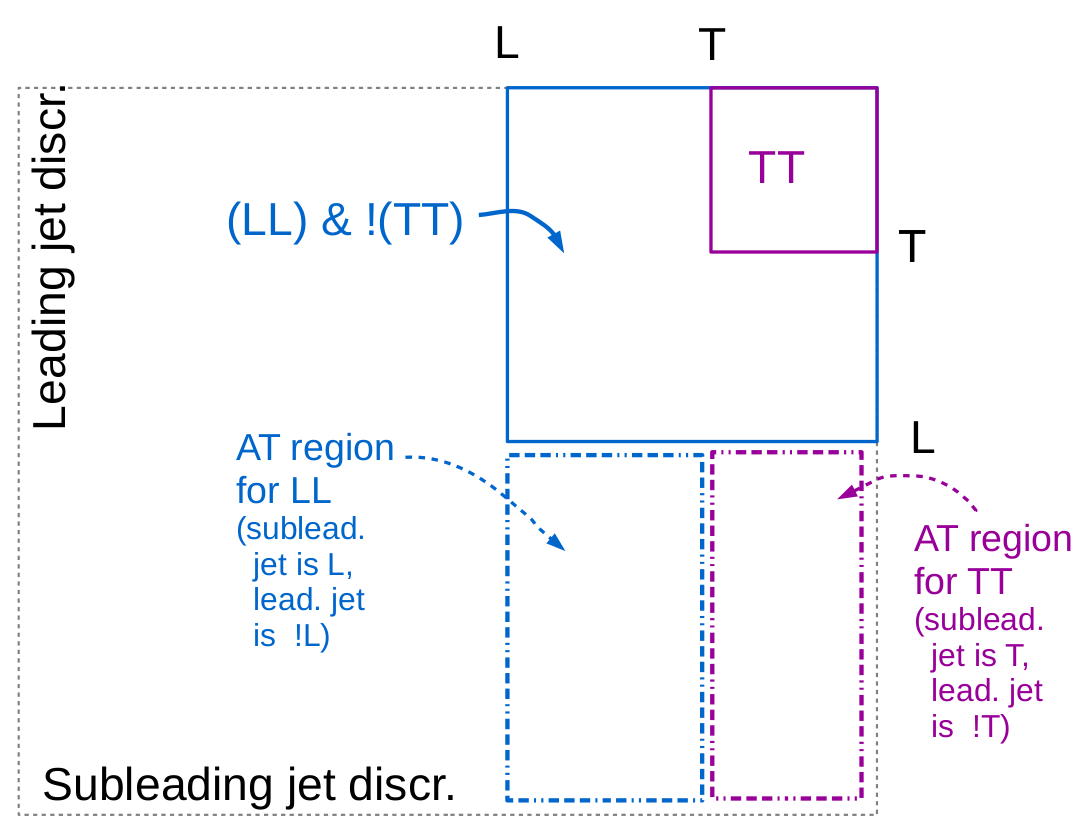
\includegraphics[width=0.6\textwidth]{Figures/splitting.png}
	\caption{A pictorial representation of the semaphoring of Loose Loose and Tight Tight events.}
	\label{fig:splitting}
\end{figure}
\clearpage

\subsection{MC distributions before applying Selections\label{ss:beforeDist}}
The kinematic variables before the application of $H \to bb$ tagger(s), are shown in Figs.\ref{fig:prePtlead} through \ref{fig:preMred}. Here, the $\ttbar$ distributions are normalized to luminosity where signal and qcd is normalized to $\ttbar$ for ease of viewing. Also, the difference between TT and LL distributions is in the weight used for each. Since the deepTagMD$\_$HbbvsQCD tagger has not been applied yet, we do not split the plots into Tight Tight and Loose Loose.

\begin{figure}[!htb]
	\centering
	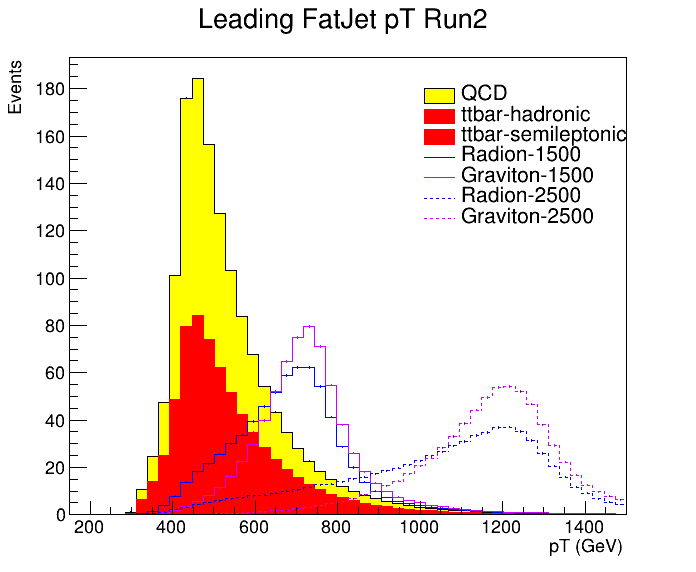
\includegraphics[width=0.4\textwidth]{Figures/pt0TT_Run2_deepTagMD_HbbvsQCD.png}
	% \includegraphics[width=0.4\textwidth]{Figures/pt021_Run2_deepTagMD_HbbvsQCD.png}
	\caption{Pre deepTagMD$\_$HbbvsQCD selection $p_T$ distribution of leading fat jet}
	\label{fig:prePtlead}
\end{figure}
\begin{figure}[!htb]
	\centering
	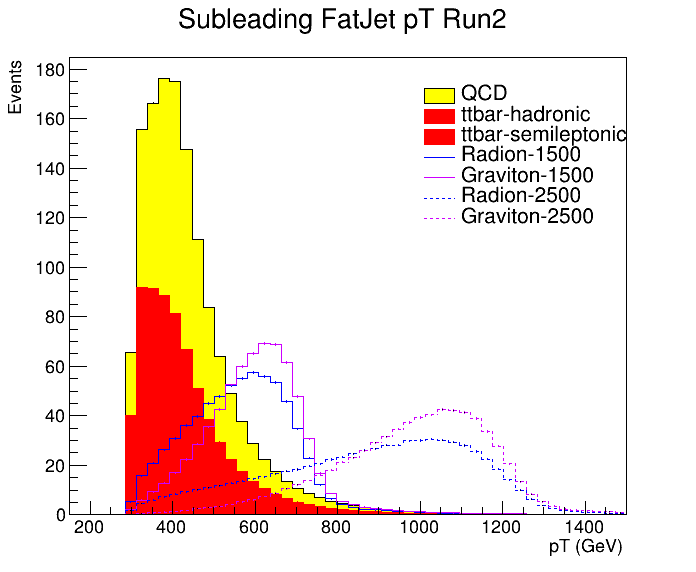
\includegraphics[width=0.4\textwidth]{Figures/pt1TT_Run2_deepTagMD_HbbvsQCD.png}
	\caption{Pre deepTagMD$\_$HbbvsQCD selection $p_T$ distribution of subleading fat jet}
	\label{fig:prePtsub}
\end{figure}
% \begin{figure}[!htb]
% 	\centering
% 	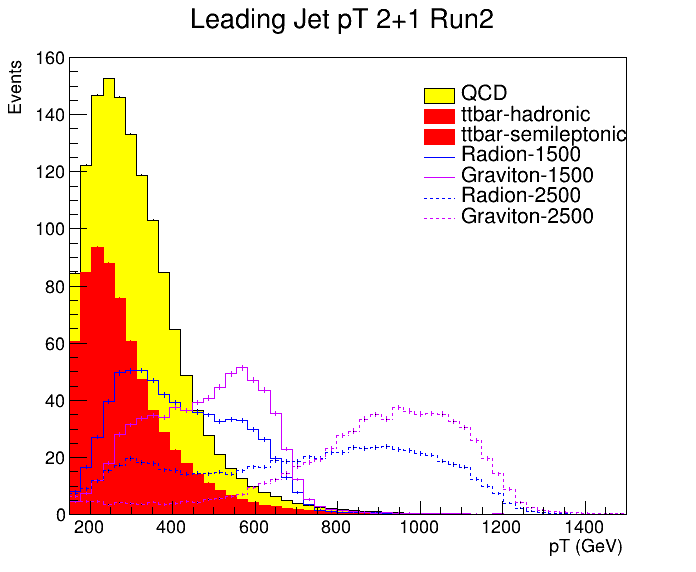
\includegraphics[width=0.4\textwidth]{Figures/bpt021_Run2_deepTagMD_HbbvsQCD.png}
% 	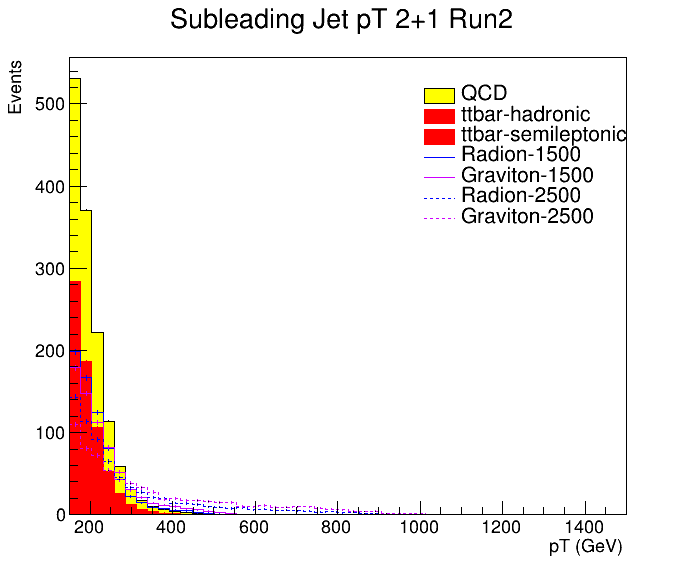
\includegraphics[width=0.4\textwidth]{Figures/bpt121_Run2_deepTagMD_HbbvsQCD.png}
% 	\caption{Pre deepTagMD$\_$HbbvsQCD selection $p_T$ distribution of leading and subleading jet for Semi-resolved.}
% 	\label{fig:prePtlead}
% \end{figure}
\begin{figure}[!htb]
	\centering
	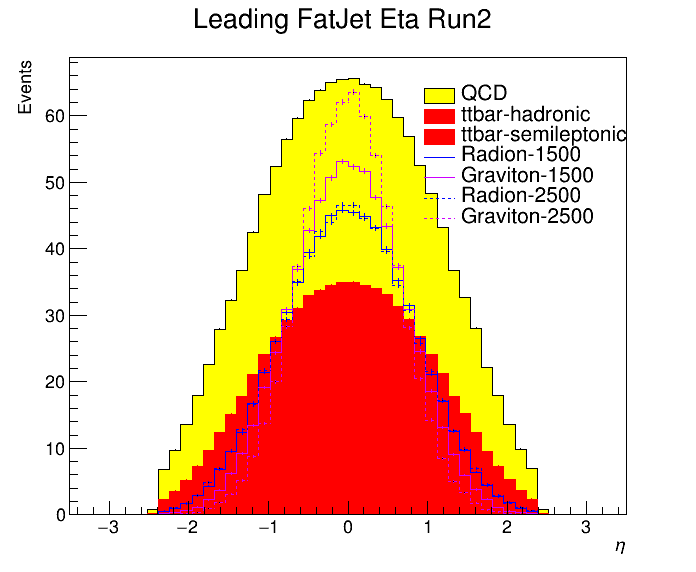
\includegraphics[width=0.4\textwidth]{Figures/eta0TT_Run2_deepTagMD_HbbvsQCD.png}
	% \includegraphics[width=0.4\textwidth]{Figures/eta021_Run2_deepTagMD_HbbvsQCD.png}
	\caption{Pre deepTagMD$\_$HbbvsQCD selection $\eta$ distribution of leading fat jet}
	\label{fig:preEtalead}
\end{figure}
\begin{figure}[!htb]
	\centering
	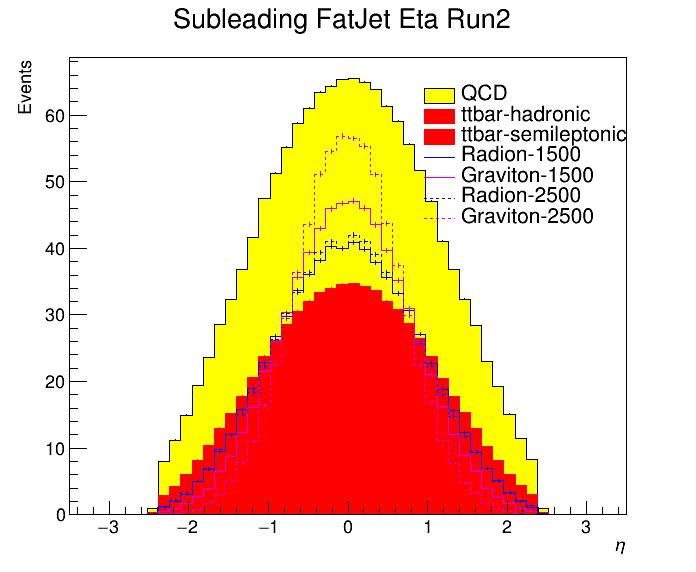
\includegraphics[width=0.4\textwidth]{Figures/eta1TT_Run2_deepTagMD_HbbvsQCD.png}
	\caption{Pre deepTagMD$\_$HbbvsQCD selection $\eta$ distribution of subleading fat jet}
	\label{fig:preEtasub}
\end{figure}
% \begin{figure}[!htb]
% 	\centering
% 	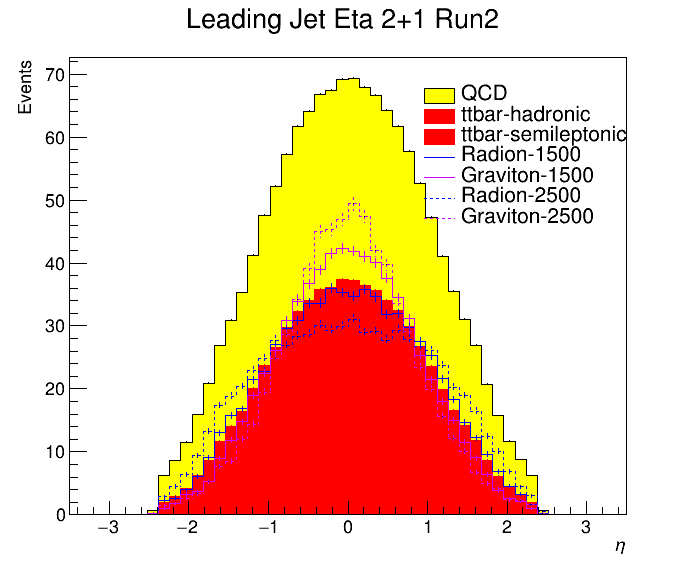
\includegraphics[width=0.4\textwidth]{Figures/beta021_Run2_deepTagMD_HbbvsQCD.png}
% 	\includegraphics[width=0.4\textwidth]{Figures/beta121_Run2_deepTagMD_HbbvsQCD.png}
% 	\caption{Pre deepTagMD$\_$HbbvsQCD selection $\eta$ distribution of leading and subleading jet for Semi-resolved.}
% 	\label{fig:prePtlead}
% \end{figure}
\begin{figure}[!htb]
	\centering
	\includegraphics[width=0.4\textwidth]{Figures/deltaEtaTT_Run2_deepTagMD_HbbvsQCD.png}
	% \includegraphics[width=0.4\textwidth]{Figures/deltaEta21_Run2_deepTagMD_HbbvsQCD.png}
	\caption{Pre deepTagMD$\_$HbbvsQCD selection $\Delta \eta$ distribution}
	\label{fig:predeltaEta}
\end{figure}
\begin{figure}[!htb]
	\centering
	\includegraphics[width=0.4\textwidth]{Figures/msd0TT_Run2_deepTagMD_HbbvsQCD.png}
	% \includegraphics[width=0.4\textwidth]{Figures/msd021_Run2_deepTagMD_HbbvsQCD.png}
	\caption{Pre deepTagMD$\_$HbbvsQCD selection $m_{j}$ distribution}
	\label{fig:premsd0}
\end{figure}
\begin{figure}[!htb]
	\centering
	\includegraphics[width=0.4\textwidth]{Figures/mred21_Run2_deepTagMD_HbbvsQCD.png}
	\includegraphics[width=0.4\textwidth]{Figures/mredTT_Run2_deepTagMD_HbbvsQCD.png}
	\caption{Pre deepTagMD$\_$HbbvsQCD selection $m_{jj}$ distribution}
	\label{fig:preMred}
\end{figure}

\section{Semi-Resolved Topology\label{app:2p1}}

The semi-resolved case bridges the gap between the fully resolved analysis for HH $\rightarrow$ 4b~\cite{CMS_AN_2015-108} and the boosted analysis, presented in Section \ref{sec:EvtSel}. It assumes one H is boosted enough to be contained within an AK8 jet with two subjets and the other H is not, resulting in two AK4 jets, one for each b quark. We use techniques similar to the boosted analysis to identify the boosted Higgs and use techniques similar to the resolved analysis to identify the two resolved b-jets. For this case, the mass range is sensitive as well.

\subsection{Event Selection\label{sec:EvtSel2p1}} 
The jet kinematics selection is the same as that of the boosted analysis for the AK8 jet. The AK4 jets also have a kinematic selection. Events are required to have:
\begin{itemize}
\item 2 AK4 jets, $p_{T}$ $>$ 30 GeV, $\etaj < 2.0$, deep Jet $>$ medium WP by year [2016:0.3093 ,2017:0.3033 ,2018:0.2770]
\item 1 AK8 jet, $p_{T}$ $>$ 300 GeV, $\etaj < 2.4$%, $\Delta$R (AK8 jet, AK4 jets) $>$ 1.5
% \item $\Delta \eta_{jjj} < 1.3$ for the leading AK8 jet and two AK4 jets, where $\Delta \eta_{jjj} = |\eta_{1stFatJet} -(\eta_{1stJet} + \eta_{2ndJet})|$.
\item Trijet mass, defined and studied in \cite{CMS-PAS-B2G-16-026}, $> 200.0$ GeV
%\item $\Delta$R of nearest unselected AK4 jet $> 1.0$ 
\end{itemize}
We choose the appropriate AK4 jets by requiring that the AK8 jet is at least $\Delta R > 0.8$ away from the candidate AK4 jets. We also require that the AK4 jets are $\Delta \phi > \frac{\pi}{2}$ away from the candidate AK8 jet in order to guarantee that the AK4 jets are in a different hemisphere than the AK8 jet. For each candidate AK4 jet pair, we require that the jets are within $\Delta R < 1.5$. After this, the dijet mass is required to be between 90 and 140 GeV, and the DeepAK8-discriminant is used to determine the control region (DeepAK8 discriminant $<$ 0.9, Tight WP) and signal region (DeepAK8 discriminant $>$ 0.9). 

\subsection{Identification of Higgs jets in semi-resolved analysis\label{sec:EvtSelBtagging}}
For the semi-resolved analysis, events are required to have at least one jet as described Section~\ref{sec:EvtSel}. The DeepAK8-tagger described in Section~\ref{sec:EvtSel} is used to identify the boosted Higgs jet in the semi-resolved analysis, requiring the fatjet pass the working point of DeepAK8 discriminant $>$ 0.9. 
We show the cutflow diagram here.
\begin{figure}[!htb]
	\centering
	\includegraphics[width=0.8\textwidth]{Figures/QCD_cutflow21_Run2_deepTagMD_HbbvsQCD.png}
	\caption{Cutflow Diagram for Semi-resolved for QCD Selection}
	\label{fig:21Cutflowqcd}
\end{figure}
\begin{figure}[!htb]
	\centering
    \includegraphics[width=0.8\textwidth]{Figures/ttbar_cutflow21_Run2_deepTagMD_HbbvsQCD.png}
	\caption{Cutflow Diagram for Semi-resolved for $\ttbar$ Selection}
	\label{fig:21Cutflowtt}
\end{figure}
\begin{figure}[!htb]
	\centering
    \includegraphics[width=0.8\textwidth]{Figures/radnar1500_cutflow21_Run2_deepTagMD_HbbvsQCD.png}
	\caption{Cutflow Diagram for Semi-resolved for Radion 1500 GeV Selection}
	\label{fig:21Cutflowsig}
\end{figure}

The invariant mass of all three jets is used in the same way as the reduced dijet mass is used for the boosted analysis and is given by:
\begin{equation}
M^{red}_{jjj} = M_{jjj} - (M_{Fatjet} - M_H) - (M_{jj(Ak4jets)} - M_H) \label{eq:mred2p1}
\end{equation} 
%\printbibliography[title={References}]
%\end{refsection}
%
%\begin{refsection}[myrefs.bib]
\chapter{Extensions of the HH4b Search}
\label{chap:six}
%\printbibliography[title={References}]
%\end{refsection}
%
%\begin{refsection}[myrefs.bib]
\chap{Conclusions}
\label{chap:conclusion}

%\printbibliography[title={References}]
%\end{refsection}
%
%%%%% BACK MATTER %%%%%
%
%%% BIBLATEX BIBLIOGRAPHY %%%
%\footnotesize
\printbibliography[title={References},heading=bibintoc]
%
%%% BIBTEX BIBLIOGRAPHY %%%
%
% Use the IEEEtran.bst style file (bibtex)
%\bibliographystyle{IEEEtran}
%
% Name the bibliography
%\setbibref{References}
% Point to bibfile
%\footnotesize\bibliography{IEEEabrv,classics}
%\bibliography{IEEEabrv,classics}
%
% APPENDICES
\begin{appendices}
% Appendix I
\chapter{}
\label{append}

\section{Statistical Tests}
\begin{figure}[!htb]
	\centering
	\includegraphics[width=0.75\textwidth]{Figures/gof_plot.pdf}
	\caption{Full Run 2 Goodness of Fit test plot with 500 toys.}
	\label{fig:gofplot}
\end{figure}

\begin{figure}[!htb]
	\centering
	\includegraphics[width=0.75\textwidth]{Figures/correlation_matrix.png}
	\caption{Full Run 2 Correlation Matrix.}
	\label{fig:corrMatrixplot}
\end{figure}


\begin{figure}[!htb]
	\centering
	\includegraphics[width=0.4\textwidth]{Figures/signalInjection0_500_sigpull_1000.png}
	\includegraphics[width=0.4\textwidth]{Figures/signalInjection0_500_sigstrength_1000.png}
	\includegraphics[width=0.4\textwidth]{Figures/signalInjection1_500_sigpull_1000.png}
	\includegraphics[width=0.4\textwidth]{Figures/signalInjection1_500_sigstrength_1000.png}
	\includegraphics[width=0.4\textwidth]{Figures/signalInjection3_500_sigpull_1000.png}
	\includegraphics[width=0.4\textwidth]{Figures/signalInjection3_500_sigstrength_1000.png}
	\caption{Signal Injection (Left Column is Pull and Right is Strength) for Full Run 2 at 1 TeV for r = 0, 1, 3 with 500 toys.}
	\label{fig:signalInjection1000plot}
\end{figure}

\begin{figure}[!htb]
	\centering
	\includegraphics[width=0.4\textwidth]{Figures/signalInjection0_500_sigpull_2000.png}
	\includegraphics[width=0.4\textwidth]{Figures/signalInjection0_500_sigstrength_2000.png}
	\includegraphics[width=0.4\textwidth]{Figures/signalInjection1_500_sigpull_2000.png}
	\includegraphics[width=0.4\textwidth]{Figures/signalInjection1_500_sigstrength_2000.png}
	\includegraphics[width=0.4\textwidth]{Figures/signalInjection3_500_sigpull_2000.png}
	\includegraphics[width=0.4\textwidth]{Figures/signalInjection3_500_sigstrength_2000.png}
	\caption{Signal Injection (Left Column is Pull and Right is Strength) for Full Run 2 at 2 TeV for r = 0, 1, 3 with 500 toys.}
	\label{fig:signalInjection2000plot}
\end{figure}

\begin{figure}[!htb]
	\centering
	\includegraphics[width=0.4\textwidth]{Figures/signalInjection0_500_sigpull_3000.png}
	\includegraphics[width=0.4\textwidth]{Figures/signalInjection0_500_sigstrength_3000.png}
	\includegraphics[width=0.4\textwidth]{Figures/signalInjection1_500_sigpull_3000.png}
	\includegraphics[width=0.4\textwidth]{Figures/signalInjection1_500_sigstrength_3000.png}
	\includegraphics[width=0.4\textwidth]{Figures/signalInjection3_500_sigpull_3000.png}
	\includegraphics[width=0.4\textwidth]{Figures/signalInjection3_500_sigstrength_3000.png}
	\caption{Signal Injection (Left Column is Pull and Right is Strength) for Full Run 2 at 3 TeV for r = 0, 1, 3 with 500 toys.}
	\label{fig:signalInjection3000plot}
\end{figure}
It is obvious that there may be some bias at the 2 and 3 TeV points when we inject $r = 0$. However, this is actually due to there being poor statistics at those mass points. When we simulate a higher integrated luminosity we get a plot with a more reasonable shape.
\begin{figure}[!htb]
	\centering
	\includegraphics[width=0.5\textwidth]{Figures/signalInjection0_500_sigpull_2000_HIGHYIELD.png}
	\caption{Signal Injection for Full Run 2 at 2 TeV for r = 0 with 500 toys and a simulated higher integrated luminosity.}
	\label{fig:signalInjection2000plotHIGH}
\end{figure}
\clearpage
\subsection{F-Test}
We performed an F-test to optimize the function used to perform the fit. The results show that a 2nd order in $\mjred$ and 2nd order in $\mred$ fit function is most optimal. 
\begin{figure}[!htb]
	\centering
	% \includegraphics[width=0.4\textwidth]{Figures/ftest_vs_FTESTpol02_pol12_notoys.pdf}
	\includegraphics[width=0.4\textwidth]{Figures/ftest_vs_FTESTBNEWpol11_pol12_notoys.pdf}
	\includegraphics[width=0.4\textwidth]{Figures/ftest_vs_FTESTBNEWpol11_pol21_notoys.pdf}
	\includegraphics[width=0.4\textwidth]{Figures/ftest_vs_FTESTBNEWpol12_pol13_notoys.pdf}
	\includegraphics[width=0.4\textwidth]{Figures/ftest_vs_FTESTBNEWpol12_pol22_notoys.pdf}
	\includegraphics[width=0.4\textwidth]{Figures/ftest_vs_FTESTBNEWpol21_pol22_notoys.pdf}
	\includegraphics[width=0.4\textwidth]{Figures/ftest_vs_FTESTBNEWpol22_pol23_notoys.pdf}
	\includegraphics[width=0.4\textwidth]{Figures/ftest_vs_FTESTBNEWpol22_pol32_notoys.pdf}
	\caption{F-test plots showing that the 2x2 fit function is the most optimal. When reading these plot, p1 is the base fit function and p2 is the function that is being compared as an improvement. Whether for p1 or p2, the designation pol gives the 
	order of the polynomial fit function in $\mjred$, $\mred$ in order. Pol11 means 1st order polynomial in $\mjred$ and 1st order polynomial in $\mred$.}
	\label{fig:ftest_plots}
\end{figure} 
% \begin{figure}[!htb]
% 	\centering
% 	\includegraphics[width=1\textwidth]{Figures/postfit_projx_fitb_2x2TT.pdf}
% 	\includegraphics[width=1\textwidth]{Figures/postfit_projx_fitb_2x2LL.pdf}
% 	\caption{Full Run 2 Tight Tight background only fits for $M_j$ axis and $M_{jj}^{red}$ axis including expected Radion 1500 GeV signal, normalized to the signal strength found by the fit.}
% 	\label{fig:ftest_fits}
% \end{figure}
\clearpage
\section{2D Alphabet Validation Study}
We are interested in knowing how well the 2D Alphabet method compares to the previous method used in \cite{CMS-PAS-B2G-16-026}. Here we present multiple limits:
\begin{itemize}
	\item The 2016 Double B tagger limit from \cite{CMS-PAS-B2G-16-026}.
	\item The 2016 Double B tagger limit made by using 2Dalphabet in 1D and including the $\tau_{21}$ cut.
	% \item The 2016 Double B tagger limit from \cite{CMS-PAS-B2G-16-026} but scaled by $\sqrt(luminosity)$.
	\item The 2016 Double B Tagger limit made with 2D Alphabet.
	\item The full run 2 Double B Tagger limit made with 2D Alphabet
	\item The full run 2 dak8MDHbb limit made with 2D Alphabet
\end{itemize}
We present the comparison in the following plot:
\begin{figure}[!htb]
	\centering
	\includegraphics[width=0.5\textwidth]{Figures/limits_HH_combine_137fb_fullrun2_limit_comparison_RadNar.png}
	\caption{Comparison plot of various limits.}
	\label{fig:compplot}
\end{figure}
\section{Example Combine Card}
The combine cards for this analysis are stored in git and may be viewed here: \\
\url{https://github.com/dbrehm/JHUanalyzer/tree/rdfHH4b/Framework/AnalysisModules/B2G-20-004/DataCards}

\section{$\tau_{21}$ Study}
We studied the effect of the $\tau_{21}$ cut used in the original analysis. We plot the results of this study:
\begin{figure}[!htb]
	\centering
	\includegraphics[width=0.4\textwidth]{Figures/limits_combine_137fb_dak8MDHbb_signalsAll_RadNar_750rmcut_yestau21.png}
	\includegraphics[width=0.4\textwidth]{Figures/limits_combine_137fb_dak8MDHbb_signalsAll_RadNar_750rmcut_notau21.png}
	\caption{Comparison of limits with and without $\tau_{21}$ cut. The plot on the right is with the cut and the plot on the left is without the cut.}
	\label{fig:tau21study}
\end{figure}
It is easy to see here that there is very little difference in the above plots. This is helpful because we then gain on statistics and systematic uncertainties as the $\tau_{21}$ scale factor uncertainty is not applied to the above limit plots.
\pagebreak
\section{By Year Fits}
Previous version of this analysis fit each year by itself. The current version of the fitting procedure combined each year so that there are only the three regions to be fit. These are the plots generated when the fit was done by year. 
\\
\textbf{These plots don't necessarily correspond to the latest fixes/updates/optimizations that were made to the full run 2 fit. Until we are able to confirm that the by year fit can happen with our latest methodology, the plots in this
section should be considered to be in need of fixing.} \\
% \subsection{Closure Test in Data\label{ss:BkgValInDataByYear}}
% \begin{figure}[!htb]
% 	\centering
% 	\includegraphics[width=1\textwidth]{Figures/postfit_projx_fitb_16CR.png}
% 	\includegraphics[width=1\textwidth]{Figures/postfit_projy_fitb_16CR.png}
% 	\caption{2016 CR fits for $M_j$ axis and $M_{jj}$ axis.}
% 	\label{fig:16CR}
% \end{figure}
% \begin{figure}[!htb]
% 	\centering
% 	\includegraphics[width=1\textwidth]{Figures/postfit_projx_fitb_17CR.png}
% 	\includegraphics[width=1\textwidth]{Figures/postfit_projy_fitb_17CR.png}
% 	\caption{2017 CR background fits for $M_j$ axis and $M_{jj}$ axis.}
% 	\label{fig:17CR}
% \end{figure}
% \begin{figure}[!htb]
% 	\centering
% 	\includegraphics[width=1\textwidth]{Figures/postfit_projx_fitb_18CR.png}
% 	\includegraphics[width=1\textwidth]{Figures/postfit_projy_fitb_18CR.png}
% 	\caption{2018 CR background fits for $M_j$ axis and $M_{jj}$ axis.}
% 	\label{fig:18CR}
% \end{figure}
\subsection{Signal Regions Prediction By Year\label{ss:BkgInSigRegionByYear}}
\begin{figure}[!htb]
	\centering
	\includegraphics[width=1\textwidth]{Figures/postfit_projx_fits_16LL.png}
	\includegraphics[width=1\textwidth]{Figures/postfit_projy_fits_16LL.png}
	\caption{2016 Loose Loose background fits for $M_j$ axis and $M_{jj}^{red}$ axis including expected Radion 1500 GeV signal, normalized to the signal strength found by the fit.}
	\label{fig:16LL}
\end{figure}
\begin{figure}[!htb]
	\centering
	\includegraphics[width=1\textwidth]{Figures/postfit_projx_fits_16TT.png}
	\includegraphics[width=1\textwidth]{Figures/postfit_projy_fits_16TT.png}
	\caption{2016 Tight Tight background fits for $M_j$ axis and $M_{jj}^{red}$ axis including expected Radion 1500 GeV signal, normalized to the signal strength found by the fit.}
	\label{fig:16TT}
\end{figure}
\begin{figure}[!htb]
	\centering
	\includegraphics[width=1\textwidth]{Figures/postfit_projx_fits_1621.png}
	\includegraphics[width=1\textwidth]{Figures/postfit_projy_fits_1621.png}
	\caption{2016 2$+$1 background fits for $M_j$ axis and $M_{jj}^{red}$ axis including expected Radion 1500 GeV signal, normalized to the signal strength found by the fit.}
	\label{fig:1621}
\end{figure}
\begin{figure}[!htb]
	\centering
	\includegraphics[width=1\textwidth]{Figures/postfit_projx_fits_17LL.png}
	\includegraphics[width=1\textwidth]{Figures/postfit_projy_fits_17LL.png}
	\caption{2017 Loose Loose background fits for $M_j$ axis and $M_{jj}^{red}$ axis including expected Radion 1500 GeV signal, normalized to the signal strength found by the fit.}
	\label{fig:17LL}
\end{figure}
\begin{figure}[!htb]
	\centering
	\includegraphics[width=\textwidth]{Figures/postfit_projx_fits_17TT.png}
	\includegraphics[width=1\textwidth]{Figures/postfit_projy_fits_17TT.png}
	\caption{2017 Tight Tight background fits for $M_j$ axis and $M_{jj}^{red}$ axis including expected Radion 1500 GeV signal, normalized to the signal strength found by the fit.}
	\label{fig:17TT}
\end{figure}
\begin{figure}[!htb]
	\centering
	\includegraphics[width=1\textwidth]{Figures/postfit_projx_fits_1721.png}
	\includegraphics[width=1\textwidth]{Figures/postfit_projy_fits_1721.png}
	\caption{2017 2$+$1 background fits for $M_j$ axis and $M_{jj}^{red}$ axis including expected Radion 1500 GeV signal, normalized to the signal strength found by the fit.}
	\label{fig:1721}
\end{figure}
\begin{figure}[!htb]
	\centering
	\includegraphics[width=1\textwidth]{Figures/postfit_projx_fits_18LL.png}
	\includegraphics[width=1\textwidth]{Figures/postfit_projy_fits_18LL.png}
	\caption{2018 Loose Loose background fits for $M_j$ axis and $M_{jj}^{red}$ axis including expected Radion 1500 GeV signal, normalized to the signal strength found by the fit.}
	\label{fig:18LL}
\end{figure}
\begin{figure}[!htb]
	\centering
	\includegraphics[width=1\textwidth]{Figures/postfit_projx_fits_18TT.png}
	\includegraphics[width=1\textwidth]{Figures/postfit_projy_fits_18TT.png}
	\caption{2018 Tight Tight background fits for $M_j$ axis and $M_{jj}^{red}$ axis including expected Radion 1500 GeV signal, normalized to the signal strength found by the fit.}
	\label{fig:18TT}
\end{figure}
\begin{figure}[!htb]
	\centering
	\includegraphics[width=1\textwidth]{Figures/postfit_projx_fits_1821.png}
	\includegraphics[width=1\textwidth]{Figures/postfit_projy_fits_1821.png}
	\caption{2018 2$+$1 background fits for $M_j$ axis and $M_{jj}^{red}$ axis including expected Radion 1500 GeV signal, normalized to the signal strength found by the fit.}
	\label{fig:1821}
\end{figure}
\begin{figure}[!htb]
	\centering
	\includegraphics[width=0.75\textwidth]{Figures/nuisance_pulls_byYear.pdf}
	\caption{Full Run 2 Nuissance Pulls Plot.}
	\label{fig:nuissancesAppend}
\end{figure}
\begin{figure}[!htb]
	\centering
	\includegraphics[width=0.75\textwidth]{Figures/impacts_byYear.pdf}
	\caption{Full Run 2 Impacts plot.}
	\label{fig:ImpactsplotAppend}
\end{figure}
\begin{figure}[!htb]
	\centering
	\includegraphics[width=1\textwidth]{Figures/postfit_projy_fits_log_16LL.png}
	\caption{2016 Loose Loose background fit for $M_{jj}^{red}$ log-scale axis including expected Radion 1500 GeV signal, normalized to the signal strength found by the fit.}
	\label{fig:16LLlog}
\end{figure}
\begin{figure}[!htb]
	\centering
	\includegraphics[width=1\textwidth]{Figures/postfit_projy_fits_log_16TT.png}
	\caption{2016 Tight Tight background fits for $M_{jj}^{red}$ log-scale axis including expected Radion 1500 GeV signal, normalized to the signal strength found by the fit.}
	\label{fig:16TTlog}
\end{figure}
\begin{figure}[!htb]
	\centering
	\includegraphics[width=1\textwidth]{Figures/postfit_projy_fits_log_17LL.png}
	\caption{2017 Loose Loose background fits for $M_{jj}^{red}$ log-scale axis including expected Radion 1500 GeV signal, normalized to the signal strength found by the fit.}
	\label{fig:17LLlog}
\end{figure}
\begin{figure}[!htb]
	\centering
	\includegraphics[width=1\textwidth]{Figures/postfit_projy_fits_log_17TT.png}
	\caption{2017 Tight Tight background fits for $M_{jj}^{red}$ log-scale axis including expected Radion 1500 GeV signal, normalized to the signal strength found by the fit.}
	\label{fig:17TTlog}
\end{figure}
\begin{figure}[!htb]
	\centering
	\includegraphics[width=1\textwidth]{Figures/postfit_projy_fits_log_18LL.png}
	\caption{2018 Loose Loose background fits for $M_{jj}^{red}$ log-scale axis including expected Radion 1500 GeV signal, normalized to the signal strength found by the fit.}
	\label{fig:18LLlog}
\end{figure}
\begin{figure}[!htb]
	\centering
	\includegraphics[width=1\textwidth]{Figures/postfit_projy_fits_log_18TT.png}
	\caption{2018 Tight Tight background fits for $M_{jj}^{red}$ log-scale axis including expected Radion 1500 GeV signal, normalized to the signal strength found by the fit.}
	\label{fig:18TTlog}
\end{figure}
\clearpage
\subsection{MC distributions before applying Selections\label{ss:beforeDistbyYear}}
The kinematic variables before the application of H->bb tagger(s), are shown in Figs.\ref{fig:prePtlead} through \ref{fig:preMred}. Here, the distributions are normalized to luminosity and the signal is normalized to 50\%. Also, the difference between TT and LL distributions is in the weight used for each. Since the deepTagMD$\_$HbbvsQCD tagger has not been applied yet, these differences may be small and not show up in these plots.
\begin{figure}[!htb]
	\centering
	\includegraphics[width=0.4\textwidth]{Figures/pt0LL_16_deepTagMD_HbbvsQCD.png}
	\includegraphics[width=0.4\textwidth]{Figures/pt0LL_17_deepTagMD_HbbvsQCD.png}
	\includegraphics[width=0.4\textwidth]{Figures/pt0LL_18_deepTagMD_HbbvsQCD.png}
	\includegraphics[width=0.4\textwidth]{Figures/pt0TT_16_deepTagMD_HbbvsQCD.png}
	\includegraphics[width=0.4\textwidth]{Figures/pt0TT_17_deepTagMD_HbbvsQCD.png}
	\includegraphics[width=0.4\textwidth]{Figures/pt0TT_18_deepTagMD_HbbvsQCD.png}
	\caption{Pre deepTagMD$\_$HbbvsQCD selection $p_T$ distribution of leading jet}
	\label{fig:prePtleadBY}
\end{figure}
\begin{figure}[!htb]
	\centering
	\includegraphics[width=0.4\textwidth]{Figures/pt1LL_16_deepTagMD_HbbvsQCD.png}
	\includegraphics[width=0.4\textwidth]{Figures/pt1LL_17_deepTagMD_HbbvsQCD.png}
	\includegraphics[width=0.4\textwidth]{Figures/pt1LL_18_deepTagMD_HbbvsQCD.png}
	\includegraphics[width=0.4\textwidth]{Figures/pt1TT_16_deepTagMD_HbbvsQCD.png}
	\includegraphics[width=0.4\textwidth]{Figures/pt1TT_17_deepTagMD_HbbvsQCD.png}
	\includegraphics[width=0.4\textwidth]{Figures/pt1TT_18_deepTagMD_HbbvsQCD.png}
	\caption{Pre deepTagMD$\_$HbbvsQCD selection $p_T$ distribution of subleading jet}
	\label{fig:prePtsubBY}
\end{figure}
\begin{figure}[!htb]
	\centering
	\includegraphics[width=0.4\textwidth]{Figures/eta0LL_16_deepTagMD_HbbvsQCD.png}
	\includegraphics[width=0.4\textwidth]{Figures/eta0LL_17_deepTagMD_HbbvsQCD.png}
	\includegraphics[width=0.4\textwidth]{Figures/eta0LL_18_deepTagMD_HbbvsQCD.png}
	\includegraphics[width=0.4\textwidth]{Figures/eta0TT_16_deepTagMD_HbbvsQCD.png}
	\includegraphics[width=0.4\textwidth]{Figures/eta0TT_17_deepTagMD_HbbvsQCD.png}
	\includegraphics[width=0.4\textwidth]{Figures/eta0TT_18_deepTagMD_HbbvsQCD.png}
	\caption{Pre deepTagMD$\_$HbbvsQCD selection $\eta$ distribution of leading jet}
	\label{fig:preEtaleadBY}
\end{figure}
\begin{figure}[!htb]
	\centering
	\includegraphics[width=0.4\textwidth]{Figures/eta1LL_16_deepTagMD_HbbvsQCD.png}
	\includegraphics[width=0.4\textwidth]{Figures/eta1LL_17_deepTagMD_HbbvsQCD.png}
	\includegraphics[width=0.4\textwidth]{Figures/eta1LL_18_deepTagMD_HbbvsQCD.png}
	\includegraphics[width=0.4\textwidth]{Figures/eta1TT_16_deepTagMD_HbbvsQCD.png}
	\includegraphics[width=0.4\textwidth]{Figures/eta1TT_17_deepTagMD_HbbvsQCD.png}
	\includegraphics[width=0.4\textwidth]{Figures/eta1TT_18_deepTagMD_HbbvsQCD.png}
	\caption{Pre deepTagMD$\_$HbbvsQCD selection $\eta$ distribution of subleading jet}
	\label{fig:preEtasubBY}
\end{figure}
\begin{figure}[!htb]
	\centering
	\includegraphics[width=0.4\textwidth]{Figures/deltaEtaLL_16_deepTagMD_HbbvsQCD.png}
	\includegraphics[width=0.4\textwidth]{Figures/deltaEtaLL_17_deepTagMD_HbbvsQCD.png}
	\includegraphics[width=0.4\textwidth]{Figures/deltaEtaLL_18_deepTagMD_HbbvsQCD.png}
	\includegraphics[width=0.4\textwidth]{Figures/deltaEtaTT_16_deepTagMD_HbbvsQCD.png}
	\includegraphics[width=0.4\textwidth]{Figures/deltaEtaTT_17_deepTagMD_HbbvsQCD.png}
	\includegraphics[width=0.4\textwidth]{Figures/deltaEtaTT_18_deepTagMD_HbbvsQCD.png}
	\caption{Pre deepTagMD$\_$HbbvsQCD selection $\Delta \eta$ distribution}
	\label{fig:predeltaEtaBY}
\end{figure}
\begin{figure}[!htb]
	\centering
	\includegraphics[width=0.4\textwidth]{Figures/msd0LL_16_deepTagMD_HbbvsQCD.png}
	\includegraphics[width=0.4\textwidth]{Figures/msd0LL_17_deepTagMD_HbbvsQCD.png}
	\includegraphics[width=0.4\textwidth]{Figures/msd0LL_18_deepTagMD_HbbvsQCD.png}
	\includegraphics[width=0.4\textwidth]{Figures/msd0TT_16_deepTagMD_HbbvsQCD.png}
	\includegraphics[width=0.4\textwidth]{Figures/msd0TT_17_deepTagMD_HbbvsQCD.png}
	\includegraphics[width=0.4\textwidth]{Figures/msd0TT_18_deepTagMD_HbbvsQCD.png}
	\caption{Pre deepTagMD$\_$HbbvsQCD selection $m_{j}$ distribution}
	\label{fig:premsd0BY}
\end{figure}
\begin{figure}[!htb]
	\centering
	\includegraphics[width=0.4\textwidth]{Figures/mredLL_16_deepTagMD_HbbvsQCD.png}
	\includegraphics[width=0.4\textwidth]{Figures/mredLL_17_deepTagMD_HbbvsQCD.png}
	\includegraphics[width=0.4\textwidth]{Figures/mredLL_18_deepTagMD_HbbvsQCD.png}
	\includegraphics[width=0.4\textwidth]{Figures/mredTT_16_deepTagMD_HbbvsQCD.png}
	\includegraphics[width=0.4\textwidth]{Figures/mredTT_17_deepTagMD_HbbvsQCD.png}
	\includegraphics[width=0.4\textwidth]{Figures/mredTT_18_deepTagMD_HbbvsQCD.png}
	\caption{Pre deepTagMD$\_$HbbvsQCD selection $m_{jj}$ distribution}
	\label{fig:preMredBY}
\end{figure}
\clearpage
\section{Limits by Year}
\begin{figure}[!htb]
	\centering
	\includegraphics[width=0.4\textwidth]{Figures/limits_combine_35_9fb_dak8MDHbb_signals16_RadNar.png}
	\includegraphics[width=0.4\textwidth]{Figures/limits_combine_45_5fb_dak8MDHbb_signals17_RadNar.png}
	\includegraphics[width=0.4\textwidth]{Figures/limits_combine_59_6fb_dak8MDHbb_signals18_RadNar.png}
	\caption{2016,2017,2018 Radion Limits for 1+1 and 2+1 using the Deep AK8 Mass Decorrelated Hbb Tagger.}
	\label{fig:RadionLimit161718}
\end{figure}

\begin{figure}[!htb]
	\centering
	\includegraphics[width=0.4\textwidth]{Figures/limits_combine_35_9fb_dak8MDHbb_signals16_GravNar.png}
	\includegraphics[width=0.4\textwidth]{Figures/limits_combine_45_5fb_dak8MDHbb_signals17_GravNar.png}
	\includegraphics[width=0.4\textwidth]{Figures/limits_combine_59_6fb_dak8MDHbb_signals18_GravNar.png}
	\caption{2016,2017,2018 Graviton Limits for 1+1 and 2+1 using the Deep AK8 Mass Decorrelated Hbb Tagger.}
	\label{fig:GravitonLimit161718}
\end{figure}
\clearpage
\section{Deep AK8 MD Hbb Tagger Working Point Study}
The following study was conducted to optimize the working points for the boosted and semi-resolved analysis since official working points are not available for this tagger. We scan the deepAK8 score and find that we should choose a working point as close to $1$ as possible without totally eliminating the background in order to do a background estimate. 
We originally chose 0.95 for the TT working point but ended up relaxing it to 0.9 because of the extreme nature of the cut. Here we present just the 1500 GeV mass point for Narrow Radion and Bulk Graviton but the other mass points have the same conclusion. We also do the same study with just \ttbar as a background to make sure the same conclusion is reached, which it is.
\begin{figure}[!htb]
	\centering
	\includegraphics[width=0.5\textwidth]{Figures/wp_RadNar1500.png}
	\includegraphics[width=0.5\textwidth]{Figures/wp_GravNar1500.png}
	\caption{Optimization of dak8MDHbb tagger using $S/\sqrt{B}$ for Narrow Radion and Bulk Graviton 1500 Gev.}
	\label{fig:SoversqrtBstudy}
\end{figure}
\begin{figure}[!htb]
	\centering
	\includegraphics[width=0.5\textwidth]{Figures/wp_RadNar1500_ttbar.png}
	\includegraphics[width=0.5\textwidth]{Figures/wp_GravNar1500_ttbar.png}
	\caption{Optimization of dak8MDHbb tagger using $S/\sqrt{B}$ for Narrow Radion and Bulk Graviton 1500 Gev with just \ttbar as a background.}
	\label{fig:SoversqrtBstudyttbar}
\end{figure}
\clearpage
\section{Trigger Scale Factor}
In previous version of this analysis, the trigger efficiency in data was used to correct the trigger response in MC. The latest method is documented in \ref{s:trigger}. Here we show the comparison of the two methods.
\begin{figure}[!htb]
	\centering
	\includegraphics[width=0.5\textwidth]{Figures/triggerMethodComparisonstudy2016.png}
	\caption{Comparison of trigger scale factors for 2016.}
	\label{fig:triggerStudy16}
\end{figure}
\begin{figure}[!htb]
	\centering
	\includegraphics[width=0.5\textwidth]{Figures/triggerMethodComparisonstudy2017.png}
	\caption{Comparison of trigger scale factors for 2017.}
	\label{fig:triggerStudy17}
\end{figure}
\begin{figure}[!htb]
	\centering
	\includegraphics[width=0.5\textwidth]{Figures/triggerMethodComparisonstudy2018.png}
	\caption{Comparison of trigger scale factors for 2018.}
	\label{fig:triggerStudy18}
\end{figure}
\clearpage
\section{Jet Energy Resolution Template Examples\label{s:jerExamples}}
Here we show example Jet Energy and Mass correction templates of both resolution and scale for Radion at 1500 GeV and $\ttbar$, for the year 2016 and the TT region as an example. 
\begin{figure}[!htb]
	\centering
	\includegraphics[width=0.4\textwidth]{Figures/Uncertainty_16_RadNar-1500_jer16failX.png}
	\includegraphics[width=0.4\textwidth]{Figures/Uncertainty_16_RadNar-1500_jer16passX.png}
	\includegraphics[width=0.4\textwidth]{Figures/Uncertainty_16_RadNar-1500_jer16failY.png}
	\includegraphics[width=0.4\textwidth]{Figures/Uncertainty_16_RadNar-1500_jer16passY.png}
	\caption{2016 Narrow Radion 1500 GeV JER pass and fail templates for $M_j$ axis and $M_{jj}^{red}$ axis.}
	\label{fig:jerRadion1}
\end{figure}
\begin{figure}[!htb]
	\centering
	\includegraphics[width=0.4\textwidth]{Figures/Uncertainty_16_ttbar_smoothed_1_2_jer16failX.png}
	\includegraphics[width=0.4\textwidth]{Figures/Uncertainty_16_ttbar_smoothed_1_2_jer16passX.png}
	\includegraphics[width=0.4\textwidth]{Figures/Uncertainty_16_ttbar_smoothed_1_2_jer16failY.png}
	\includegraphics[width=0.4\textwidth]{Figures/Uncertainty_16_ttbar_smoothed_1_2_jer16passY.png}
	\caption{2016 $\ttbar$ JER pass and fail templates for $M_j$ axis and $M_{jj}^{red}$ axis.}
	\label{fig:jerttbar1}
\end{figure}

\begin{figure}[!htb]
	\centering
	\includegraphics[width=0.4\textwidth]{Figures/Uncertainty_16_RadNar-1500_jes16failX.png}
	\includegraphics[width=0.4\textwidth]{Figures/Uncertainty_16_RadNar-1500_jes16passX.png}
	\includegraphics[width=0.4\textwidth]{Figures/Uncertainty_16_RadNar-1500_jes16failY.png}
	\includegraphics[width=0.4\textwidth]{Figures/Uncertainty_16_RadNar-1500_jes16passY.png}
	\caption{2016 Narrow Radion 1500 GeV JES pass and fail templates for $M_j$ axis and $M_{jj}^{red}$ axis.}
	\label{fig:jesRadion2}
\end{figure}
\begin{figure}[!htb]
	\centering
	\includegraphics[width=0.4\textwidth]{Figures/Uncertainty_16_ttbar_smoothed_1_2_jes16failX.png}
	\includegraphics[width=0.4\textwidth]{Figures/Uncertainty_16_ttbar_smoothed_1_2_jes16passX.png}
	\includegraphics[width=0.4\textwidth]{Figures/Uncertainty_16_ttbar_smoothed_1_2_jes16failY.png}
	\includegraphics[width=0.4\textwidth]{Figures/Uncertainty_16_ttbar_smoothed_1_2_jes16passY.png}
	\caption{2016 $\ttbar$ JES pass and fail templates for $M_j$ axis and $M_{jj}^{red}$ axis.}
	\label{fig:jesttbar2}
\end{figure}

\begin{figure}[!htb]
	\centering
	\includegraphics[width=0.4\textwidth]{Figures/Uncertainty_16_RadNar-1500_jmr16failX.png}
	\includegraphics[width=0.4\textwidth]{Figures/Uncertainty_16_RadNar-1500_jmr16passX.png}
	\includegraphics[width=0.4\textwidth]{Figures/Uncertainty_16_RadNar-1500_jmr16failY.png}
	\includegraphics[width=0.4\textwidth]{Figures/Uncertainty_16_RadNar-1500_jmr16passY.png}
	\caption{2016 Narrow Radion 1500 GeV JMR pass and fail templates for $M_j$ axis and $M_{jj}^{red}$ axis.}
	\label{fig:jerRadionAppend}
\end{figure}
\begin{figure}[!htb]
	\centering
	\includegraphics[width=0.4\textwidth]{Figures/Uncertainty_16_ttbar_smoothed_1_2_jmr16failX.png}
	\includegraphics[width=0.4\textwidth]{Figures/Uncertainty_16_ttbar_smoothed_1_2_jmr16passX.png}
	\includegraphics[width=0.4\textwidth]{Figures/Uncertainty_16_ttbar_smoothed_1_2_jmr16failY.png}
	\includegraphics[width=0.4\textwidth]{Figures/Uncertainty_16_ttbar_smoothed_1_2_jmr16passY.png}
	\caption{2016 $\ttbar$ JMR pass and fail templates for $M_j$ axis and $M_{jj}^{red}$ axis.}
	\label{fig:jerttbarAppend}
\end{figure}

\begin{figure}[!htb]
	\centering
	\includegraphics[width=0.4\textwidth]{Figures/Uncertainty_16_RadNar-1500_jms16failX.png}
	\includegraphics[width=0.4\textwidth]{Figures/Uncertainty_16_RadNar-1500_jms16passX.png}
	\includegraphics[width=0.4\textwidth]{Figures/Uncertainty_16_RadNar-1500_jms16failY.png}
	\includegraphics[width=0.4\textwidth]{Figures/Uncertainty_16_RadNar-1500_jms16passY.png}
	\caption{2016 Narrow Radion 1500 GeV JMS pass and fail templates for $M_j$ axis and $M_{jj}^{red}$ axis.}
	\label{fig:jesRadionAppend}
\end{figure}
\begin{figure}[!htb]
	\centering
	\includegraphics[width=0.4\textwidth]{Figures/Uncertainty_16_ttbar_smoothed_1_2_jms16failX.png}
	\includegraphics[width=0.4\textwidth]{Figures/Uncertainty_16_ttbar_smoothed_1_2_jms16passX.png}
	\includegraphics[width=0.4\textwidth]{Figures/Uncertainty_16_ttbar_smoothed_1_2_jms16failY.png}
	\includegraphics[width=0.4\textwidth]{Figures/Uncertainty_16_ttbar_smoothed_1_2_jms16passY.png}
	\caption{2016 $\ttbar$ JMS pass and fail templates for $M_j$ axis and $M_{jj}^{red}$ axis.}
	\label{fig:jesttbarAppend}
\end{figure}
\clearpage
\section{$\mred$ Dependent $\Delta \eta_{jj}$ Cut studies\label{s:mredDeltaEta}}
We studied the effect on both the signal efficiency and the limits of introducing a $\mred$ dependent $\Delta \eta_{jj}$ cut in order to try to capture any lost signal, particularly at higher resonance masses.
We concluded that although the signal efficiency for each region and resonance mass point increases, it does not do so enough to make a difference in the expected limits and therefore we do not implement this change.
\begin{figure}[!htb]
	\centering
	\includegraphics[width=0.5\textwidth]{Figures/sigEffrad_combined_Run2_deepTagMD_HbbvsQCD_base.png}
	\caption{Radion Signal Efficiency for full Run 2.}
	\label{fig:sigEffRad}
\end{figure}
\begin{figure}[!htb]
	\centering
	\includegraphics[width=0.5\textwidth]{Figures/sigEffgrav_combined_Run2_deepTagMD_HbbvsQCD_base.png}
	\caption{Radion Signal Efficiency for full Run 2.}
	\label{fig:sigEffGrav}
\end{figure}

\begin{figure}[!htb]
	\centering
	\includegraphics[width=0.5\textwidth]{Figures/sigEffrad_combined_Run2_deepTagMD_HbbvsQCD_mred.png}
	\caption{Radion Signal Efficiency for full Run 2 with $\mred$ Dependent $\Delta \eta_{jj}$ Cut.}
	\label{fig:sigEffRadmred}
\end{figure}
\begin{figure}[!htb]
	\centering
	\includegraphics[width=0.5\textwidth]{Figures/sigEffgrav_combined_Run2_deepTagMD_HbbvsQCD_mred.png}
	\caption{Radion Signal Efficiency for full Run 2 with $\mred$ Dependent $\Delta \eta_{jj}$ Cut.}
	\label{fig:sigEffGravmred}
\end{figure}
\begin{figure}[!htb]
	\centering
	\includegraphics[width=0.5\textwidth]{Figures/limits_HH_combine_137fb_deltaEtaComparison_RadNar_fixedmredDeltaEtaCheckRadion.pdf}
	\caption{Full Run 2 Radion Limit comparison with $\mred$ Dependent $\Delta \eta_{jj}$ Cut.}
	\label{fig:RadionLimitFULLmred}
\end{figure}

\begin{figure}[!htb]
	\centering
	\includegraphics[width=0.5\textwidth]{Figures/limits_HH_combine_137fb_deltaEtaComparison_GravNar_fixedmredDeltaEtaCheckGraviton.pdf}
	\caption{Full Run 2 Graviton Limit comparison with $\mred$ Dependent $\Delta \eta_{jj}$ Cut.}
	\label{fig:GravitonLimitFULLmred}
\end{figure}
\clearpage
\section{Wide Resonances}
We perform this analysis for resonances with a higher width as a check of the validity of the background estimate. Here we show both the unblinded results for the bulk graviton and radion signal samples with a 10\% width. 
\begin{figure}[!htb]
	\centering
	\includegraphics[width=1\textwidth]{Figures/postfit_projx_fits_LLwide.pdf}
	\caption{Full Run 2 Loose Loose fits for $M_j$ axis including expected Radion 2000 GeV wide signal, normalized to the signal strength found by the fit.}
	\label{fig:LLmjwide}
\end{figure}
\begin{figure}[!htb]
	\centering
	\includegraphics[width=1\textwidth]{Figures/postfit_projy_fits_LLwide.pdf}
	\caption{Full Run 2 Loose Loose fits for $M_{jj}^{red}$ axis including expected Radion 2000 GeV wide signal, normalized to the signal strength found by the fit.}
	\label{fig:LLmjjwide}
\end{figure}
\begin{figure}[!htb]
	\centering
	\includegraphics[width=1\textwidth]{Figures/postfit_projx_fits_TTwide.pdf}
	\caption{Full Run 2 Tight Tight fits for $M_j$ axis including expected Radion 2000 GeV wide signal, normalized to the signal strength found by the fit.}
	\label{fig:TTmjwide}
\end{figure}
\begin{figure}[!htb]
	\centering
	\includegraphics[width=1\textwidth]{Figures/postfit_projy_fits_TTwide.pdf}
	\caption{Full Run 2 Tight Tight fits for $M_{jj}^{red}$ axis including expected Radion 2000 GeV wide signal, normalized to the signal strength found by the fit.}
	\label{fig:TTmjjwide}
\end{figure}
\begin{figure}[!htb]
	\centering
	\includegraphics[width=1\textwidth]{Figures/postfit_projx_fits_21wide.pdf}
	\caption{Full Run 2 2$+$1 fits for $M_j$ axis including expected Radion 2000 GeV wide signal, normalized to the signal strength found by the fit.}
	\label{fig:21mjwide}
\end{figure}
\begin{figure}[!htb]
	\centering
	\includegraphics[width=1\textwidth]{Figures/postfit_projy_fits_21wide.pdf}
	\caption{Full Run 2 2$+$1 fits for $M_{jj}^{red}$ axis including expected Radion 2000 GeV wide signal, normalized to the signal strength found by the fit.}
	\label{fig:21mjjwide}
\end{figure}
\begin{figure}[!htb]
	\centering
	\includegraphics[width=1\textwidth]{Figures/nuisance_pulls_wide.pdf}
	\caption{Full Run 2 Nuissance Pulls Plot for 2 TeV wide Radion signal.}
	\label{fig:nuissanceswide}
\end{figure}

\begin{figure}[!htb]
	\centering
	\includegraphics[width=0.75\textwidth]{Figures/gof_plot_wide.pdf}
	\caption{Full Run 2 Goodness of Fit test plot with 500 toys for 2 TeV wide Radion signal.}
	\label{fig:gofplotwide}
\end{figure}
\begin{figure}[!htb]
	\centering
	\includegraphics[width=0.75\textwidth]{Figures/correlation_matrix_wide.png}
	\caption{Full Run 2 Correlation Matrix for 2 TeV wide Radion signal.}
	\label{fig:corrMatrixplotwide}
\end{figure}
\begin{figure}[!htb]
	\centering
	\includegraphics[width=0.4\textwidth]{Figures/signalInjection0_500_sigpull_1000wide.png}
	\includegraphics[width=0.4\textwidth]{Figures/signalInjection0_500_sigstrength_1000wide.png}
	\includegraphics[width=0.4\textwidth]{Figures/signalInjection1_500_sigpull_1000wide.png}
	\includegraphics[width=0.4\textwidth]{Figures/signalInjection1_500_sigstrength_1000wide.png}
	\includegraphics[width=0.4\textwidth]{Figures/signalInjection3_500_sigpull_1000wide.png}
	\includegraphics[width=0.4\textwidth]{Figures/signalInjection3_500_sigstrength_1000wide.png}
	\caption{Wide Signal (Left Column is Pull and Right is Strength) Injection for Full Run 2 at 1 TeV for r = 0, 1, 3 with 500 toys.}
	\label{fig:signalInjection1000plotwide}
\end{figure}

\begin{figure}[!htb]
	\centering
	\includegraphics[width=0.4\textwidth]{Figures/signalInjection0_500_sigpull_2000wide.png}
	\includegraphics[width=0.4\textwidth]{Figures/signalInjection0_500_sigstrength_2000wide.png}
	\includegraphics[width=0.4\textwidth]{Figures/signalInjection1_500_sigpull_2000wide.png}
	\includegraphics[width=0.4\textwidth]{Figures/signalInjection1_500_sigstrength_2000wide.png}
	\includegraphics[width=0.4\textwidth]{Figures/signalInjection3_500_sigpull_2000wide.png}
	\includegraphics[width=0.4\textwidth]{Figures/signalInjection3_500_sigstrength_2000wide.png}
	\caption{Wide Signal (Left Column is Pull and Right is Strength) Injection for Full Run 2 at 2 TeV for r = 0, 1, 3 with 500 toys.}
	\label{fig:signalInjection2000plotwide}
\end{figure}

\begin{figure}[!htb]
	\centering
	\includegraphics[width=0.4\textwidth]{Figures/signalInjection0_500_sigpull_3000wide.png}
	\includegraphics[width=0.4\textwidth]{Figures/signalInjection0_500_sigstrength_3000wide.png}
	\includegraphics[width=0.4\textwidth]{Figures/signalInjection1_500_sigpull_3000wide.png}
	\includegraphics[width=0.4\textwidth]{Figures/signalInjection1_500_sigstrength_3000wide.png}
	\includegraphics[width=0.4\textwidth]{Figures/signalInjection3_500_sigpull_3000wide.png}
	\includegraphics[width=0.4\textwidth]{Figures/signalInjection3_500_sigstrength_3000wide.png}
	\caption{Wide Signal (Left Column is Pull and Right is Strength) Injection for Full Run 2 at 3 TeV for r = 0, 1, 3 with 500 toys.}
	\label{fig:signalInjection3000plotwide}
\end{figure}
% Appendix II
\include{text/13-appendix-ii}
\end{appendices}
%
%%% CV %%%
% \include{text/15-my-original-cv}
%
%%% Biographical Sketch %%%
% \include{text/16-biographical-sketch}
%
\end{document}